%!TEX root = ../Report.tex
\chapter{The causes of higher housing costs}\label{chap:the-causes-of-higher-housing-costs}

There are many reasons housing prices have increased so rapidly over the past two decades.

Economic changes -- largely welcome -- increased how much people are prepared to pay for housing.
Household incomes have grown, credit is more available following financial deregulation, and nominal interest rates are lower, partly as a result of inflation targeting.

Tax and welfare settings have encouraged people to buy their own homes and to invest in housing.
Tax settings have made home-ownership attractive relative to renting, and housing investments attractive relative to other investments.
And demand has been fuelled by leverage cycles and market sentiment expecting house prices to keep going up.

There are also more people wanting to be housed.
The population has grown particularly rapidly over the past decade, after immigration jumped in the mid-2000s.
And there are more overseas investors -- although they have probably also increased supply.

In the short run, any unexpected increase in demand raises prices, because it takes many months to build new housing.%
	\footcites{RBA2014SubmissionAffordableHousingInquiry}{RBAStatementonMonetaryPolicyFeb17}{HousingAus17}
But over the long run, rising demand won't result in much higher house prices if more housing can be built.%
	\footcites{RBA2014SubmissionAffordableHousingInquiry}[][4]{Glaeser-2013-Natio-of-gamblers}
Rapid population growth in Australia in the 1950s was matched by record rates of home building,%
    \footcite{Eslake2013}
and house prices barely moved.

But over much of the last two decades, constraints have limited new supply that would normally respond to higher demand. Planning rules that restrict the construction of more homes in inner and middle ring suburbs have dragged on development. Not enough medium-density housing, such as mid-rise and low-rise apartments, townhouses and terraces, has been built in the established suburbs of our major cities closest to most new jobs and existing infrastructure. Although there have been more high-rise apartments, overall dwelling supply has not matched population growth, resulting in higher prices.

Construction has picked up in recent years, especially in the middle ring of Sydney. But building has only just reached the level required given population growth, while community opposition is mounting.

\section{Strong demand for housing has contributed to rising prices }\label{sec:strong-demand-for-housing-has-contributed-to-rising-prices}

Many factors have contributed to rising housing demand from both investors and owner-occupiers.%
	\footcites{Yates}{ABSHousingFinanceAustraliaAugust2017}
This section explains them:

\begin{itemize}
\item
Strong economic growth and rising household incomes;
\item
Falling interest rates and more readily available credit;
\item
The geographic shift of jobs -- and therefore demand for accommodation -- towards large capital cities, particularly their centres;
\item
Tax and welfare settings encouraging home-ownership, including first-home buyers assistance, and the exclusion of family homes from capital gains tax, Age Pension assets test, and state land tax;
\item
Tax settings encouraging investment in housing, particularly the capital gains tax discount and negative gearing arrangements;
\item
Tax settings that discourage downsizing;
\item
High rates of immigration;
\item
More foreigners responding to global economic factors by investing in Australian housing; and
\item
A self-reinforcing cycle of increased prices and leverage.
\end{itemize}

\subsection{Economic changes allow Australians to spend more on housing }\label{subsec:economic-changes-allow-australians-to-spend-more-on-housing}

A variety of economic changes led to Australian households being prepared to pay more to own their own home.

Australian households have benefited from \textbf{strong economic growth}.
Median equivalised household income increased by more than 60 per cent in real terms over the past two decades.
In part this reflects rising income per hour worked.%
\footcites{AusProdTrends17}{EslakeWalsh-2011-Aust-Prod-challenge}
And in part it reflects rising workforce participation,%
    \footcites{YatesExplainer2015}{AGoodHouse2008}
particularly of women.%
	\footcite{Borland-June-2017-snapshot}

As they became richer, households devoted a greater proportion of their growing incomes to larger, higher-quality and better-located homes.%
	\footnote{See \Vref{sec:were-spending-more-on-housing}.}
And people also chose to live in \textbf{smaller households} (see \Vref{fig:household-size-projections}).
Strong economic growth also boosted confidence that house prices would continue to grow.

As \textbf{interest rates fell,} Australian households could afford to borrow more to pay more for housing. \emph{Official} interest rates fell as a result of inflation targeting from the mid-1990s.
Interest rates \emph{paid} also fell as a result of financial deregulation in the 1980s and 1990s, which compressed bank margins.%
	\footcites{Lowe2017Householddebt}{2010BirdsEyeView}
The decline in interest rates meant that a given monthly mortgage repayment could support a loan of twice the size, and so people bid up the price of houses.%
	\footcites{KellyHarrisonHunterEtAl2013}{Ellis2013-Housing-Mortgage-Markets-speech}{InterestRatesandHosuePrices}{KohlerandvanderMerwe}{OttoGrowthofHousePrices}
Consequently, household borrowing and house prices became a much larger multiple of household incomes.%
	\footcites{KellyHarrisonHunterEtAl2013}{KohlerandvanderMerwe}
Australia is not alone: lower interest rates across the globe have increased house prices in most countries.%
	\footnote{\textcite{InterestRatesandHosuePrices} found that short-term interest rates are an important driver of house prices in most countries. \textcite{SecularDrivers2015} found that the long-term decline in global interest rates is due to weaker global economic growth, population ageing, higher inequality globally, and precautionary saving in emerging markets.}

Australia is becoming a more \textbf{services and knowledge-based economy}, which is concentrating economic activity, jobs, and demand for accommodation into a relatively small area, increasing housing demand in Australia's large cities, and especially their inner suburbs (see \Vref{fig:house-prices-cities-regions} and \Vref{fig:house-prices-within-cities}).

\phantomsection\label{paragraph:cities-increase-incomes}
Australia is already highly urbanised by world standards, with more of its people in its two biggest cities than any other country in the OECD.%
    \footcite{OECD2014OECDFactbook2014}
The shift of economic activity and population towards major cities and their surrounds is continuing notwithstanding a once-in-a-century mining boom.%
    \footcite{DaleyWoodChivers2017RegPatterns}
Cities tend to be more productive, as is reflected in higher wages, GDP and rates of innovation per person.%
    \footcite{Romer-cities}
Large-city populations and jobs are continuing to grow as the economy continues to shift from manufacturing and agriculture to business and other services.%
    \footcite{Daley-productivity-geography}
Official population projections expect these trends to continue.%
    \footcites{ABS2013PopulationprojectionsAustralia}[][21]{IA_2018_Future_cities}
Again, these are global trends.%
	\footnote{According to \textcite{SuperstarCities} people are attracted to `superstar' cities -- a definition which covers most large Australian cities -- that offer high-paying jobs and good amenity, and this pushes up house prices. Larger cities tend to have higher house prices as well-located land becomes more valuable. \textcite{EllisAndrewsRBA2001}.}
While the crowding and congestion of very large cities might one day encourage more population growth in Australia's regions, this has not yet happened in international cities much larger than Sydney and Melbourne.

Within major cities, jobs are concentrating towards their centre.\footcites{Jackson_2018_id_where_are_the_jobs}{SGS2017jobscities}
Between 2006 and 2011, half of all jobs growth was  within the city centres and inner suburbs in both Melbourne and Sydney (\Vref{fig:jobs-growth-cbds}).%
	\footnote{Melbourne residents in suburbs more than 20 kilometres from the CBD have fewer than three jobs nearby for every 10 residents, while those close to the city centre have access to nine jobs for every 10 residents: \textcite{KellyDonegan2015-City-limits}.}
Knowledge-intensive businesses -- which tend to be the most productive, and which are growing fastest -- particularly benefit from clustering together in the centres of large cities.%
	\footcite[][23--29]{KellyDonegan2015-City-limits}

\begin{figure}
\caption{Most jobs growth between 2006 and 2011 was in city centres}\label{fig:jobs-growth-cbds}
\units{Net employment growth, Sydney and Melbourne, thousands}
\includenextfigure{atlas/Charts-for-housing-affordability-report.pdf}
\noteswithsources{For definitions of inner, middle and outer suburbs, see \textcite{BITRE14-15}}
{Grattan analysis; \textcite{BITRE14-15}}
\end{figure}

Melbourne is Australia's most highly centralised city.
New medium-sized and large businesses mainly choose to locate in Melbourne's CBD and its immediate surrounds, or close to the airport.%
	\footcite{Rasmussen-economic-geography}
Meanwhile, most of Melbourne's middle and outer suburbs had fewer companies with turnover of more than \$1~million in 2016 than in 2011.

Because many of the additional jobs are being created towards large city centres, residential land close by has become more desirable.
As a result, dwelling prices have risen faster in the inner-city than in outer suburbs (\Vref{fig:house-prices-within-cities}).

\subsection{High immigration boosted demand for housing, particularly in major cities }\label{subsec:high-immigration-boosted-demand-for-housing-particularly-in-major-cities}
\CenturyFootnote

Strong population growth, both from natural increase and overseas migration, has increased demand for housing and contributed to the increase in dwelling prices, particularly in our major cities.%
    \footnote{\textcites{RBA2015SubmissionHomeOwnershipInquiry}{CommissionMigrantIntake2016}. There is also international evidence that immigration can contribute to higher house prices, particularly if the supply of new housing is constrained (as is the case in Australia). For example%
    , \textcite{AndrewsEtAlHousing} conclude that migration tends to initially translate into higher real house
prices in the short to medium run, particularly when new housing supply is inelastic. \textcite{Gonzalez_2013_spain_house_prices} found that immigration accounted for roughly one-third of the increase in Spanish housing prices over the period 1998-2008.}

Australia's population increased by 3.8~million between 2006 and 2016.
Most of the increase is housed in the major cities.
Melbourne's population grew from 3.6~million to 4.5~million people between 2006 and 2016, while Sydney's grew by 700,000 to 4.6~million.%
    \footnote{Using `Significant Urban Area' geographical classification from \textcite{ABS-2017-regionalpopgrowth}.}
Strong interstate migration has also contributed to population growth in Melbourne in recent years.
The Australian Bureau of Statistics (ABS) forecasts that Australia's population will grow to around 38~million by 2050.%
	\footcite[][Series~B]{ABS2013PopulationprojectionsAustralia}

Immigration has been the major driver of population growth since the mid-2000s (\Vref{fig:pop-growth-cities}).
Since 2005, annual net overseas migration has averaged 200,000 people per year, up from 100,000 in the decade prior.
    \footcite{ABS-2016-Aust-Demographic-stats}
More temporary migrants, mainly students and skilled workers, contributed to much of the increase in net overseas migration.%
    \footnote{Most temporary skilled workers came to Australia under the 457 visa, which was introduced in 1996 (\textcite[][11]{Philipsmigrationstats2010}).
    The 457 visa is uncapped and is used by Australian businesses to fill vacancies when there is a recognised skills shortage. Skilled migration (both temporary and permanent), and uncapped migration from New Zealand, grew faster when Australia's mining boom economy grew faster than almost all other developed economies.  
    In combination with  increasing demand for higher education from Asia, student visa changes and universities seeking more international students, Australia became more attractive for international students due to changes to permanent migration policies that favoured former international students (\textcite[][23]{Norton2016MappingAustralianhigher}).}

\begin{figure}
\caption{Population growth has been strong since the mid-2000s, especially in major capital cities}\label{fig:pop-growth-cities}
\includenextfigure{atlas/Charts-for-housing-affordability-report.pdf}
\noteswithsources{There is a series break in the September quarter 2006 when the `net overseas migration' definition was changed to include people living in Australia for 12 months out of a 16-month period (12/16 method), rather than 12 months out of 12 months (12/12 method). The ABS estimates that the change in methodology to the 12/16 method results in net overseas migration being about 25 per cent higher than under the 12/12 method. See \textcites{ABS_2016_1415_explanatory_note}{Morrison-2017-Missing-million-is-Aust-migration-actually-high}{Murray-2017-Finding-Australias-missing-million} for a detailed discussion.}%
{\textcites{ABS-2017-AustDemographicstats}{ABS-2017-regionalpopgrowth}}
\end{figure}

Net overseas migration had slowed from the very high levels seen in 2007-08 and 2012-13, but has recently accelerated again. In the past year the number of new overseas migrants to Melbourne and Sydney has passed its previous peak in 2008 (\Vref{fig:NOM-states}).

\begin{figure}
\caption{Overseas migration into NSW and Victoria is at the record levels seen in 2008}\label{fig:NOM-states}
\units{Four-quarter rolling annual sum, thousands of people}
\includenextfigure{atlas/Charts-for-housing-affordability-report.pdf}
\noteswithsource{There is a series break in 2006 when the `net overseas migration' definition was changed, see Notes in \Cref{fig:pop-growth-cities}}%
{\textcites{ABS-2017-AustDemographicstats}}
\end{figure}

Immigrants are more likely to move to Australia's major cities than existing residents, which increases demand for well-located housing in cities.
In 2011, 86 per cent of immigrants lived in major cities, compared to 65 per cent of the Australian-born population.%
    \footcites{CommissionMigrantIntake2016}[][24--25]{DaleyWoodChivers2017RegPatterns}
Within cities, recent immigrants are more likely than existing residents to live in apartments or in fringe suburbs.%
    \footcites[][12]{Birrellhousingaffordabilitycrisis}{SGS2017popgrowth}

The migrants who contributed to the boom in Australia's population from the mid-2000s tended to be younger than the Australian population average, and much younger than migrants in the past, as \Vref{fig:pop-generations} shows.%
  \footnote{See also \textcite[][Graph~5]{Ellis2017Kellyspeech}.}
A large and growing share of these migrants were skilled workers and international students (see \Vref{fig:NOM-categories}).
International students primarily move to inner-city areas and generally seek cheaper housing.
This may have contributed to cheaper housing rising in price by more than expensive housing.%
    \footnote{See \Vref{fig:house-price-deciles} and \Vref{fig:rents-deciles}.}

\doublecolumnfigure{
\caption{Australia's population was significantly reshaped by the \mbox{late-2000} migration wave}\label{fig:pop-generations}
\units{Australian population by age, millions}
\includenextfigure{atlas/Charts-for-housing-affordability-report.pdf}
\sources{\textcites{ABS2014Australianhistoricalpop}{ABS20016Censuspopulationhousing}}
}{
\caption{Australia's net migrant intake is expected to be 250,000 in 2020, most of whom will be temporary residents}\label{fig:NOM-categories}
\units{Net overseas migration, by visa type}
\includenextfigure{atlas/Charts-for-housing-affordability-report.pdf}
\sources{\textcites{ABS-2017-Migration-Aust-201516}{DIBP2016}.}
}


Net overseas migration is predicted to increase to 250,000 per year by 2019-20 (\Vref{fig:NOM-categories}).%
	\footnote{\textcite{DIBP2016}. Net overseas migration is composed of temporary and permanent migration. The Federal Government has a permanent migrant target of 190,000 per year, plus a humanitarian intake that averaged 15,800 over the five years to 2015-16
	(\textcite{Phillips-2017-Aust-humanitarian-program-guide-to-the-stats}).}
Changes to the temporary skilled migration program, to take effect in March 2018,%
    \footnote{\textcite{DIBP2017457changes}. The government is abolishing the 457 visa and replacing it with a  Temporary Skills Shortage (TSS) visa.}
may result in fewer skilled workers immigrating to Australia than forecast by the Department of Immigration and Border Protection in 2016.%
    \footnote{\textcites{Sherrell20184_57changes}{Birrell457changes}. 
    This already seems to be happening: 457 visa numbers fell over the year to December 2017: \textcite{457_datagovau_2018}.}
While these changes will not directly affect the uncapped foreign students program, which is driving much of the current increase in net overseas migration, they may put off some potential students who planned to transition to a 457 visa as a potential pathway towards permanent residence.\footcite{Pascoe_2018_smh_457_student_visas}
Many of the temporary migrants who add to net overseas migration in one year subsequently become permanent residents: temporary migrants receive about half of the 190,000 permanent residency visas granted each year.%
	\footnote{\textcite[][19]{DIBP-2016-Australias-migration-trends-1415}. Net arrivals of people on permanent visas accounts for 30 to 40 per cent of net overseas migration (\Cref{fig:NOM-categories}).}


House prices themselves can alter the distribution of population growth \emph{between} large cities. In recent years Melbourne's relatively cheaper land has attracted people that may have otherwise considered moving to Sydney.%
    \footnote{\textcite{RBACarrFernandesRosewall}. 
    Others may have chosen to relocate to regional NSW: \textcite{Hanna_2018_smh_sydney_migration}.}
Estimates suggest that a 10 per cent increase in Sydney prices relative to other large cities would reduce migration to Sydney by about 10,000 people per year.%
	\footnote{\textcite[][13]{NSW-Treasury-Housing-Prices-and-Migration-Flows}
	find that a 1 percentage point increase in NSW house prices relative to the rest of Australia would lower NSW's share of net overseas migration by just over 0.3 percentage points (about 600 people a year at current migration rates).
	The same relative increase in NSW house prices would also result in an outflow of around 550 persons each year in interstate migration. Modelling by the \textcite{GeographicLabourMobility} found that a 10 per cent fall in the ratio of house prices between a destination region in Australia and a source region increases the labour force migration flow by 1.8 per cent (Sydney prices increased by around 10 per cent relative to Melbourne in the four years to September 2017).}


\subsection{Government tax and welfare settings encourage people to buy homes }\label{subsec:government-policy-settings-encourage-people-to-buy-homes}

Four key policy settings in place for decades have encouraged people to own a home.
Given the non-financial benefits of home-ownership, particularly security of tenure, it is likely that many people would buy a home even without these policies.

First, owner-occupiers benefit because the family home is \textbf{exempt from capital gains tax (CGT)} and there is \textbf{no tax on imputed rents} (the value of owning a home that you live in).
These concessions combined are estimated to be worth around \$35~billion a year.%
    \footnote{\Vref{sec:any-reforms-to-the-capital-gains-tax-exemption-on-the-main-residence-should-proceed-with-caution}. See also \textcite[][23]{KellyHarrisonHunterEtAl2013}.}
They would be worth even more today given recent increases in house prices.%
    \footnote{For example, exempting owner-occupied housing liable for capital gains tax benefits home-owners to the tune of \$35 billion a year. Taxing imputed rents is worth billions more (\textcite[][88--89]{Treasury-2017-TES-for-2016}).}

Second, most of the value of the main residence is \textbf{excluded from the Age Pension assets test}.
This benefit is worth at least \$7 billion a year to home-owning pensioners.%
    \footnote{\textcite{DaleyEtAl-2013-BalancingBudgets}.
	The pension assets test effectively includes only the first \$200,000 of value of a family home, and ignores the remainder.}
The pension assets test heavily favours owner-occupiers. Many households with significant housing wealth receive a full-rate Age Pension, while many pensioners who do not own their homes get much less pension despite having less assets overall.%
    \footnote{Half of all Age Pension payments go to households with net wealth of more than \$500,000.
	One in five pension dollars go to households worth at least \$1~million: \textcites[][37]{DaleyEtAl-2013-BalancingBudgets}[][21]{Daley2017implicationsageing}. This excludes the impact of changes to the Age Pension assets test that took effect from 1 January 2017, which reduced the entitlements of 326,000 Age Pensioners.
	However these changes will only reduce overall Age Pension payments to part-rate pensioners by around \$1~billion in 2017-18, which is unlikely to substantially change the distribution of pension payments by net wealth given total Age Pension spending of \$45~billion in 2017-18. \textcites{FairerAccess2017MorrisonMediaRelease}[][6--27]{Budget2017-18-BP1}.}

Third, owner-occupied housing is \textbf{exempt from state land taxes}.
As a result, about 75 per cent of residential land by value attracts no land tax, and state government budgets forgo about \$7~billion a year in revenue.%
  \footnote{\textcite[][24]{KellyHarrisonHunterEtAl2013} updated to 2017 using \textcite[][Table~61]{ABS-aus-system-of-nat-accounts2016-17}.}

Fourth, federal and state governments have provided \textbf{financial assistance to first home buyers} in various forms for decades.%
    \footnote{\textcite{Eslake2013} identifies 1964 as the beginning of Commonwealth assistance.}
Government assistance has mainly pushed up purchase prices for first home buyers rather than making the first purchases of a home more affordable (See \Vref{fig:fhb-grants-fhb-financing}). It has been expensive: it is estimated that governments spent \$22.5~billion (in 2010-11 dollars) on grants to first home buyers between 1964 and 2011.%
    \footnote{\textcite{Eslake2013} states that, `it's hard to think of any government policy that has been pursued for so long, in the face of such incontrovertible evidence that it doesn't work, than the policy of giving cash to first home buyers'.}

\subsection{Tax settings encourage people to invest in housing}\label{subsec:tax-settings-encourage-people-to-invest-in-housing}

More recently, changes to capital gains tax in 1999 encouraged investors to buy property, increasing investor demand for housing and pushing some first home buyers out of the market.%
    \footnote{First home buyers account for less than 10 per cent of housing financing commitments, down from 20 per cent in the early 1990s, while investors account for around half of financing commitments, up from around 20 per cent. \textcites{ABSHousingFinanceAustraliaAugust2017}{Eslake-2017-causes-effects-housing-affordability}.}
In 1999, the CGT system was changed so that tax was levied on only 50 per cent of the \emph{nominal} capital gain on an asset held for more than one year.
Previously, 100 per cent of the \emph{real} capital gain was taxed.
As things turned out, over the past 18 years much less capital gains tax has been collected, because dwelling prices have risen much faster than inflation.%
	\footnote{\textcite[][10]{DaleyWood2016-Negative-Gearing-CGT}. Because inflationary gains are not `income' in a true sense, some discount on returns to savings is justified. Given inflation rates and returns in 1999, a tax on only 50 per cent of the gains was roughly equivalent to taxing only the real return. But with falling inflation and rapidly rising asset prices, the 50 per cent discount has overcompensated property investors for inflation over time.}

With capital gains taxed less than income, investors have preferred investments with strong capital returns, even if they earnt relatively little annual income.
So property investors have been willing to accept relatively little rental income in the expectation of a more lightly-taxed capital gain.%
	\footcites{RBA2015SubmissionHomeOwnershipInquiry}{DaleyWood2016-Negative-Gearing-CGT}
With strong price growth, this strategy has been largely successful over the past two decades.%
	\footcite[][9]{DaleyWood2016-Negative-Gearing-CGT}

The relatively light taxation of capital gains increased the incentives for investors to negatively gear property.
Investors can borrow to invest and deduct the interest costs against other income at their marginal rate.
The capital gains are then only taxed at half their marginal rate.%
    \footnote{In addition, they benefit because the tax deduction for the interest payments is claimed immediately,
    but the tax on the capital gain is deferred until sale.}
Since the introduction of the CGT discount, landlords have collectively paid more in interest costs than they have received in rents.
And almost all the net additional investors in property have been negatively geared.
Some 1.3~million landlords reported collective losses of \$11~billion in 2014-15.%
	\footnote{\textcite[][9, 25--26]{DaleyWood2016-Negative-Gearing-CGT}. The CGT discount and negative gearing cost the budget \$6.8~billion a year.}

Tax incentives encouraging housing investors may also explain why the prices of low-value homes have increased faster than other homes (See \Vref{fig:house-price-deciles}). Increased investor demand for housing has likely been channelled into low-value homes that are lightly taxed under states' progressive land taxes and tax-free thresholds.%
    \footnote{Progressive state land tax rate schedules and tax-free thresholds mean that higher value land and larger landholders are subject to higher rates of land tax, affecting rental yields.
    (See \Vref{fig:land-tax-investors}.)
    For example, \textcite[][21]{Wood-Ong-AHURI-2010-factors-affecting-landlords} note that booming land values have pushed residential property investors beyond land tax tax-free thresholds and into higher land tax brackets in recent years, especially in states where land tax thresholds are not indexed to rising land values. Existing research suggests the presence of investor clientele effects where housing investment is targeted at housing market segments that benefit from the most generous tax treatment (\textcite{Wood-Tu-2004-investor-clienteles-rental-housing}).}


Since 2003, self-managed super funds have also been able to borrow and invest in property, although this change has had little impact on the overall property market.%
    \footnote{Since the rule change, \$26~billion of self-managed super fund assets have been invested in residential property -- or just 0.4 per cent of the total value of Australia's \$6.6~trillion residential property market.
	SMSFs have invested a further \$74~billion in non-residential property.
	\textcites[][13]{RBA2015SubmissionHomeOwnershipInquiry}[][Asset allocation tables]{ATO-2016-Asset-allocation-tables}.
	The ALP has announced plans to reverse this policy change: \textcite{Coorey2017-AFR-housing}.}

These tax settings have encouraged investment in housing in preference to other more productive assets, dragging on economic growth.\footnote{\textcite[][15--16]{DaleyWood2016-Negative-Gearing-CGT}.}

\subsection{Tax settings discourage people from downsizing, increasing demand for well-located houses}\label{subsec:tax-settings-discourage-people-from-downsizing-increasing-demand-for-well-located-houses}

As life expectancy increases and people stay healthier, older people are staying in their homes for longer,%
	\footnote{According to the Productivity Commission,~about 20 per cent of people aged 60 or over~have sold their home and purchased a less expensive one since turning 50.
	Another 15 per cent have ``strong intentions'' to do so in future. \textcite{PC-2015-Housing-decisions-elderly}.}
even if their home is unsuitable for their needs, and has poorly utilised space.%
	\footnote{In 2016, 325,000 (13 per cent) of people aged 70 years or over without children lived in a house with four bedrooms or more: see \Vref{fig:owners-spare-bedrooms}.}
This inefficient use of the housing stock is partly a result of tax and welfare settings, but mainly the result of the failure to build more medium-density housing in established areas.

A number of tax and welfare settings discourage downsizing and more efficient use of the housing stock.
Because primary residences are not included in the Age Pension means test, pensioners may lose some or all of their pension if they downsize.
Downsizers have to pay stamp duty on any new home they buy.%
    \footnote{A number of States and Territories have exemptions specifically for seniors and pensioners: \textcite[][137]{PC-2015-Housing-decisions-elderly}.}
And earnings from the cash released by downsizing are taxed, whereas capital gains on the existing home are not.
These disincentives become more substantial as house prices rise.

However, research suggests~that for most older Australians, these financial considerations are not the dominant influences on the decision to downsize or not.

When people do move, their choice is primarily driven by lifestyle reasons and difficulty in maintaining a large house and garden (\Vref{fig:motives-for-downsizing}).%
    \footcites[][40]{PC-2015-Housing-decisions-elderly}[][81--82, 138]{JuddEtAlDownsizing2014}[][15]{Daley-2017-AAA-Housing-for-older-Australians-COTA-prez}
They look primarily for a home that will be easier to maintain, and that is close to facilities and their networks.
    \footcite[][95]{JuddEtAlDownsizing2014}
Financial considerations are much less of an issue on their minds.

And when people do not downsize, their primary problem is usually that they cannot `downsize in place' -- they can't find suitable housing in the same local area.
These considerations typically dwarf the financial trade-off between more free cash, but a lower age pension.%
	\footcite[][7]{PC-2015-Housing-decisions-elderly}
Stamp duty costs were a barrier for only about 5 per cent of those thinking about downsizing.%
    \footcite[][40]{PC-2015-Housing-decisions-elderly}
\begin{figure}
\caption{A downsized home is chosen primarily for features and location, not financial outcomes}\label{fig:motives-for-downsizing}
\units{Important considerations when moving, percentage of downsizers}
\includenextfigure{atlas/Charts-for-housing-affordability-report.pdf}
\source{\textcite[][95]{JuddEtAlDownsizing2014}}
\end{figure}

\subsection{Foreign investors have added to already strong housing demand, but have probably also increased supply}\label{subsec:foreign-investors-have-added-to-already-strong-housing-demand-but-have-also-increased-supply}

Increased investment by foreigners has increased demand for Australian housing, although it has probably also increased supply. Foreign investment in housing has also increased a lot in many other global cities such as London, New York, San Francisco and Vancouver.%
    \footcites{Surowiecki2014realestate}{UBSglobalrealestate}{Rogers_2016_foreign_investment_broken_supply}
Despite public perceptions, the best evidence is that foreign investment has only increased housing prices a little, and may well have slowed growth in rents a little.

\subsubsection{The scale of foreign investment}\label{subsec:scale-foreign-investment}

Foreign investors have become an increasingly prominent, and controversial, part of Australia's property market.

Foreign investment in residential property was  approximately 5-10 per cent of the volume of turnover in 2016-17, and 10-15 per cent of new housing construction.%
	\footnote{Based on \textcite{Fraser2017stockbroker} forecast of 15,000 approvals in 2016‑17 and adjusted according to historical number of conversions from approvals to actual purchases.
	Foreign investments in real estate must be approved by the Foreign Investment Review Board (FIRB).
	We assume that 35 per cent of approvals for developers, and 90 per cent of approvals for individuals, ultimately result in a foreign purchase (\textcite[][]{GauderHoussardOrsmond}).
    FIRB approvals accounted for 24 per cent of the value of residential real estate transactions in 2015-16 (8 per cent of the number) (\textcite{FIRB2015factsheet}).
    This amounted to \$72~billion of approvals, up from \$5-to-\$20 billion in the 2000s, and more than double the value of approvals in 2013-14 (\textcites{ABS-2017-Residential}{HassanEconomicUpdate}).
    But approvals in 2015-16 were probably boosted by one-off factors.
    Higher foreign investor application fees were imposed from December 2015, which encouraged foreign investors to bring forward applications to before December 2015.
    And prior to the December 2015 changes, investors could submit multiple applications for multiple dwellings but  not follow through with a purchase: \textcite[][13]{GauderHoussardOrsmond}.
	So from 2016-17 onwards, approvals are likely to be lower than in 2015-16, but actual foreign purchases will be closer to FIRB approvals data than in previous years (see also \textcite{Kearns2017ausproperty}).}
A number of data sources show that over recent years there are more foreign investors, particularly Chinese, in residential property in Australia.
    \footcites{NAB2017}{SMHAusHousing}[][Box~B]{RBAFinancialStability2016}{JandaForeigners}
But overall, foreigners own at most 2 per cent of the housing stock.%  

\subsubsection{Controls on foreign investment}\label{subsec:controls-foreign-investment}

Australia now regulates foreign investment in real estate more tightly than any other country (\Vref{tbl:Intl-regulation-of-foreign-real-estate-investment}). In part, these laws aim to direct foreign investment into building new houses and apartments, increasing supply of new housing, and limiting upward pressure on house prices.%
    \footcite{FIRB2017realestate}
Foreign investors cannot legally buy existing residential property in Australia. They can buy \emph{new} residential property in Australia if they receive approval from the FIRB and after paying a fee.%
    \footcite{FIRB2017residentialland}
These properties can be rented out.
Temporary residents may purchase one established property as their place of residence while in Australia if they receive FIRB approval.
And some foreign investors may become citizens over time.

About 90 per cent of the FIRB approvals for foreign investment in 2015-16 were for new housing, with the remainder for established properties (which can be purchased by temporary residents to live in while they reside in Australia).%
	\footnote{Foreign investment has become increasingly focused on new dwellings: approvals for purchases of new residential dwellings accounted for about 82 per cent of the value of all FIRB residential approvals over the past decade.}

The Commonwealth Government announced additional charges on foreign investment in the 2017 Budget, including curbs on CGT exemptions, a tax on vacant properties, and higher application fees.%
	\footnote{The Commonwealth Government announced that temporary and foreign residents will now pay capital gains tax on their main residence, unlike permanent residents (\textcite{Budget1718-Stronger-rules-foreign-investors-own-Aust-housing}).}
State governments also tax foreign investors more than other owners of residential real estate. Most states levy a stamp duty surcharge on foreign investors, and some have introduced a land tax surcharge.
Some states are also introducing a vacant property tax (see \Vref{sec:better-enforcing-existing-rules-on-foreign-investment-in-housing-could-make-housing-more-affordable}).

\begin{table*}
\renewcommand*{\arraystretch}{1.25}
\caption{Australia's laws covering foreign investment in residential real estate are strict compared to most comparable countries}\label{tbl:Intl-regulation-of-foreign-real-estate-investment}
\units{Summary of laws covering foreign investment in residential real estate}
\begin{tabularx}{\linewidth}{p{0.15\linewidth}XXXXX}
\toprule
                        & \textbf{Limit on purchase}                       & \textbf{Special taxes}                                              & \textbf{Purchase approvals}      & \textbf{Empty dwelling taxes}          & \textbf{Other}\tabularnewline
\midrule
\textbf{Australia}      & \textcolor{white}{Only new}\cellRed              & \textcolor{white}{Stamp duty and land tax in some states.
No main residence capital gains tax exemption.}\cellRed    & \textcolor{white}{Yes, with application fee}\cellRed & \textcolor{white}{Yes. Additional vacant property tax for both foreigners and locals in Victoria.}\cellRed & Withholding tax on sale\cellOrange\tabularnewline
\textbf{Canada}         & None                                             & \textcolor{white}{15 per cent tax in Vancouver and Toronto}\cellRed & \textcolor{white}{Yes}\cellRed         & Vancouver only\cellOrange      & Can only finance with Canadian bank\cellOrange\tabularnewline
\textbf{Denmark}        & Restrictions in holiday areas\cellOrange         & No                                                                  & \textcolor{white}{Yes}\cellRed         & No                             & \tabularnewline
\textbf{France}         & None                                             & Wealth tax\cellDarkOrange                                           & No                                     & Paris only\cellDarkOrange      & \tabularnewline
\textbf{Hong Kong}      & None                                             & \textcolor{white}{Higher stamp duty for foreign buyers}\cellRed   & No                                     & No                             & \tabularnewline
\textbf{New Zealand}    & \textcolor{white}{Restriction to new properties to be introduced}\cellRed       & No                                                                  & Yes if `sensitive land'\cellOrange         & No                             & Withholding tax on sale\cellOrange\tabularnewline
\textbf{Singapore}      & Apartments only\cellDarkOrange                   & \textcolor{white}{Higher stamp duty}\cellRed                        & Sometimes\cellDarkOrange               & Yes                            & \tabularnewline
\textbf{Switzerland}    & \textcolor{white}{Only one holiday home}\cellRed & No                                                                  & \textcolor{white}{Yes}\cellRed         & No                             & \textcolor{white}{Restrictions on renting out and selling in some cantons}\cellRed\tabularnewline
\textbf{United Kingdom} & None                                             & Non-resident companies pay capital gains tax\cellOrange                                     & No                                     & No                             & \tabularnewline
\textbf{USA}            & None                                             & No                                                                  & No                                     & No                             & Withholding tax on sale\cellOrange\tabularnewline
\textbf{Germany, Belgium, Netherlands, Japan, Spain} & In Spain, only residents can buy \textgreater{} \euro{}500,000 & No & No & No &\tabularnewline
\bottomrule
\end{tabularx}

\sources{\textcite{ACIL2017Property}; Grattan analysis}
\end{table*}

\subsubsection{Existing housing and foreign investors}\label{subsec:foreign-investment-existing-housing}

While official FIRB data suggests foreigners have mostly invested in new housing developments, foreigners may have in fact purchased established dwellings in contravention of Australia's foreign investment rules, contributing to higher demand, but not increasing supply.%
    \footnote{\textcite{AbacusGuestRohde} find that foreign investment in existing housing pushed up prices by more than investment in new housing.}
Numerous reports of foreign investment rules being circumvented prompted a House of Representatives Standing Committee inquiry into foreign investment in residential real estate in~2014.%
    \footnote{\textcite{Harrisinvestors}.
    More than 60 established properties illegally purchased have been forcibly sold over the past two years:  \textcite{Cadmanforiegnproperty}.}
This inquiry found evidence of a number of illegal purchases of established property, in breach of foreign investment rules. 

As a result, in December 2015 the Federal Government shifted enforcement to the Australian Taxation Office, tightened foreign investment rules further, and increased penalties.%
    \footcites{HouseofReps2014}{FIRB2015factsheet}{WallaceRealEstate}{RyanForeignInvestment}
Since these changes, the ATO has detected some 570 foreign purchasers that have broken foreign investment rules relating to residential property, leading to 61 forced property sales%
	\footcite{Morrison-2017-Govt-force-forns-sell-100M-real-estate}
-- not a particularly material issue relative to Australia's housing market of 9.3 million dwellings.

Nevertheless, suspicions remain that foreign investors are continuing to purchase established dwellings.%
    \footnote{\textcite{RogersetalChineseRealEstate}; 53 per cent of respondents disagreed with the statement `Government has effectively regulated foreign investment in greater Sydney's housing market' and 25 per cent disagreed with the statement that `Chinese investments in greater Sydney's housing market are by and large conducted legally within the foreign investment rules'.}
If foreign investors are breaching the law, this may have increased prices in some areas, particularly in Sydney and Melbourne.

\subsubsection{Price impact of foreign investment}\label{subsec:foreign-investment-prices}

The extent to which foreign investment pushes up the price of housing depends on how much foreign investment adds to both demand \emph{and} supply.%
	\footnote{How increased foreign demand affects increased supply depends on the elasticity of the supply of new housing, and these two factors then affect the price of both new housing and established housing, which are close substitutes.}
Greater foreign investor demand will lead to higher prices unless the additional supply of new housing due to foreign investors is even greater than the additional demand.

Permitting foreign investors to buy new housing obviously increases demand for housing.
But supply also increases if foreign investors enable developers to build more housing than otherwise.%
  \footcite{ACIL2017Property}
This may be because overseas investors enable developers -- often themselves foreigners -- to build larger or higher buildings. Overseas investors may be more prepared to buy new properties off the plan or be prepared to accept a lower rate of return.%
    \footnote{A lower rate of return enables a higher building because additional storeys usually cost more to build per dwelling: they require additional engineering, and take longer to construct, which adds to holding costs (\textcite[][5]{ShooryRosewall2017}).}
And overseas investors may attract overseas developers with better access to finance, or with better knowledge of new technology.%
	\footcites{Kearns2017ausproperty}{GauderHoussardOrsmond}
These factors matter more for inner-city apartment developments, which are less constrained by planning rules, and which have been the focus for foreign investors.
Apart from these markets, new housing supply is fairly inelastic in Australia (see \Vref{subsec:housing-construction-did-not-keep-pace-with-increased-demand-and-prices}).

The evidence is limited, but it seems that overall foreign investment has \emph{both} increased prices a little, and increased the supply of housing a little.

A 2016 Treasury Working Paper concluded that foreign investment pushed up prices by only a small amount between~2010 and~2015.
This paper found that foreign investment accounted for 0.5 to 1~per cent of the average increase in prices in Melbourne and Sydney (between \$80 and \$122 of the average increase in dwelling prices of \$12,800 each quarter).%
	\footnote{\textcite{Treasury2016Wokker}. This study used data from July 2010 to March 2015.}
The OECD recently concluded that foreign investment has not had a substantial impact on prices.%
    \footnote{\textcite[][29]{OECD2017c}. See also \textcite{GauderHoussardOrsmond} which came to a similar conclusion.
    In contrast, \textcite{AbacusGuestRohde} found that foreign investment accounted for 20-to-30 per cent of the increase in housing prices between 2004 and 2014 in Sydney and Melbourne.
    But there are problems with the methods in this paper.
    The authors use FIRB approvals as a proxy for foreign investment, but fail to adjust for approvals that do not result in purchases, and so overstate the impact of foreign investment on house prices.}
Nonetheless, public perception is that foreign investment is a major cause of rising house prices in recent years.%
    \footnote{A survey of Sydney residents by \textcite{RogersetalChineseRealEstate} found high levels of concern and discontent about foreign investment.
    A \textcite{McCrindleSydneyReport} report found that `81 per cent of survey respondents believe that overseas property investors are driving price increases' (41 per cent said Australian investors are contributing).
    A \textcite{DukeProperty} survey found that 60 per cent of respondents believed foreign investors caused the housing boom.
    A \textcite{LowyInstPoll} poll found that 70 per cent of respondents believe the government allows too much investment from China in Australian residential real estate.}

\subsubsection{Rental impact of foreign investment}\label{subsec:foreign-investment-rents}

Whatever its impact on asset prices, foreign investment may have a different impact on rents.
The best evidence is that it has had little effect, and if anything has probably slowed rent growth a little.
The effect on rents depends on how much of the housing purchased by foreign investors is then rented out to Australian residents.
If a foreign investor is also a migrant and lives in the purchased property themselves, they do not add to housing pressures since they would have needed to be housed anyhow.

It seems that relatively few foreign purchases are left vacant, and they are a very small proportion of the housing stock. Census data suggest that the share of vacant dwellings has increased only slightly over recent decades.%
    \footnote{Analysis of Census data by \textcite{SGSCensus2017} suggests the share of unoccupied private dwellings increased from 9-to-10 per cent in the 1980 and 1990s to 10.7 per cent in 2011 and 11.2 per cent in 2016.
	See also \textcite{Pawson-2017-theConvo-Taxing-empty-homes}.
	Others dispute the extent of vacancies, \textcite{ACIL2017Property}. According to \textcite{OECD2017housingdatabase}, vacant dwellings account for 10 per cent of Australia's dwelling stock. This is lower then the 12 per cent vacancy rate in New Zealand and 13 per cent in the USA, but Australia's vacancy rate is much higher than European countries such as Germany and Switzerland.
	By contrast, analysis of water consumption suggests that about 5 per cent of Melbourne's dwellings are left vacant (\textcite{CashmoreSpecVac}). Official rental vacancy rates -- calculated as the share of properties advertised for rent divided by the number of private rental properties in the market -- are around 2 per cent in Melbourne and Sydney.  However, these vacancy rates explicitly exclude homes that are not advertised for rent (\textcites{RENSW-vacancy-rate-2018}{REIV-vacancy-rate-2018}).}
A significant number of these vacant dwellings are holiday homes, in the process of being sold, or between tenants.

At most, properties left vacant by foreign owners would comprise less than 0.3 per cent of the housing stock.%
    \footnote{Foreigners only own 2 per cent of the housing stock, and only a fraction of this is vacant at any one time.}
Similarly, a study found that the vast majority of foreign-owned property in London is used regularly by locals, with only a small proportion used irregularly, and less than 1 per cent largely vacant.%
    \footcite{ScanlonLondon}
Nevertheless, vacancy rates are materially lower in greater Melbourne than in inner Melbourne, where there are substantially more foreign owners.%
    \footcite{SGSCensus2017}

But even if all vacant properties suspected to be owned by foreign investors were rented out, rents would only reduce a little.%
	\footcite{Murray2017a}
And if all these vacant properties were sold, house prices would be at most about 1 per cent lower than otherwise.%
	\footnote{Grattan analysis of \textcite{Abelson-and-Chung-2005-realstoryofhousingprices}.}

In reality, while some foreign-owned houses may be left vacant, many foreign investors may end up settling in Australia, or have family in Australia who use their property.
In these cases, foreign investment is just an early manifestation of demand from future migration.

Apart from increasing house prices a little, and reducing rents a little, foreign investment in housing can bring other benefits: foreign developers can bring in new techniques and skills that increase productivity in construction; and they add to government revenue.%
	\footcites{FairerAccess2017MorrisonMediaRelease}{ACIL2017Property}

\subsection{Higher leverage contributes to higher property prices}\label{subsec:financial-cycles-affect-housing}

Finally, house prices are also affected by leverage cycles and expectations of future house price increases.

Property prices usually play an important role in determining how much a household can borrow for other purposes such as funding a small business, or making other investments.
This can have a self-reinforcing effect: rapid increases in credit, particularly for mortgages, drive up property prices, which in turn increase collateral values and thus the amount of credit that households can obtain.%
    \footcites{NBER-Credit-Supply-and-House-Prices}{Bernanke-Gertler-credit-channel-1995}

Past house price cycles have seen similar patterns. Periods of strong credit growth and rapid house price appreciation have been followed by periods of stagnating prices and flat-lining housing debt.\footcite{Daley-Coates-Wiltshire-2017-InsideStory-What-comes-after-housing-boom} 

Whether leverage cycles and potentially irrational expectations of future growth in house prices lead to sustained house price falls depends on whether banks maintain good lending standards and remain well regulated (see \Vref{subsec:australias-banking-system-seems-robust-but-regulators-need-to-remain-vigilant}).%
    \footcite[][]{Glaeser-2013-Natio-of-gamblers}

\section{Supply has not kept up with growing demand, leading to higher prices}\label{sec:supply-has-not-kept-up-with-growing-demand}

House prices would not rise so far in response to rising demand if more housing could be built in our major cities where most of the additional population want to live.%
    \footnote{For example, \textcite[][325]{Glaeser-Gyourko-Can-Cheap-Credit-Explain-the-Housing-Boom} find that interest rates have a much larger impact on house prices in supply-constrained cities than where new housing supply is more responsive.
    Where housing supply is relatively elastic, increased housing demand should lead to substantially more housing construction and relatively flat house prices equal to the costs of new construction.
    And this outcome is possible: \textcite{Eslake2013} notes that the total number of homes in Australia grew faster than the Australian population in every decade until the 2000s.}
But construction has failed to keep pace with the rapid increase in demand for housing in Australia, and consequently prices rose.%
    \footnote{Of course, in the short run, there are lags in the ability of the supply of housing to respond to changes in demand, which can leave house prices temporarily higher than they would be otherwise (\textcite[][26]{KohlerandvanderMerwe}). However such lags cannot account for sustained price increases over the past two decades, or the decade-long delay in housing supply responding to increased demand.}
The primary obstacle is that planning rules delay or prevent development (see \Vref{sec:the-major-problem-is-planning-regulations}).
The story is similar in many markets around the world (\Vref{box:International-supply-literature}).



On most estimates, dwellings fell behind population growth for the decade from 2005 to 2014.\footcites{KohlerandvanderMerwe}{Gradwell2017HousingBalance}
Only in the past couple of years has construction started to get close to matching population growth; the backlog of a decade of under-supply remains.
If projections for future population growth are right, then future rates of construction will need to be even higher than at present.

When construction did increase over the past few years, a large proportion was inner-city high-rise construction in Melbourne and Brisbane.
But, inner-city areas are inherently limited, and are unlikely to provide sufficient housing for future (or even current) population growth. There has been a greater volume of medium-density development in middle-ring suburbs in Sydney, but less elsewhere.

In Sydney, there has been limited city fringe development until recently, increasing its price.
In Melbourne, Brisbane and Perth, supply on the urban fringe has been less constrained, and many new homes have been built.
But these homes are often far from jobs, and poorly served by public transport.%
    \footcites{NBER2017HsiehMoretti}{Parkhomenko2016}{Herkenhoff2017EmpireStates}

\subsection{Housing construction fell well behind increased demand from 2006}\label{subsec:housing-construction-did-not-keep-pace-with-increased-demand-and-prices}

For much of the last 15 years, housing construction did not keep up with the strong growth in demand for housing described in \Cref{sec:strong-demand-for-housing-has-contributed-to-rising-prices}. This mismatch contributed to higher housing prices.%
	\footnote{\textcite{Abelsonetal2005} found that more housing results in lower prices than otherwise in the long run. Between the 1970s and 2003, a 1 per cent increase in the housing stock per capita resulted in an estimated decrease in real house prices of around 3.5 per cent.}
The best estimate is that several years of construction -- probably at even faster rates than now -- will be needed to erode the large backlog that accumulated in the 2000s.

\doublecolumnfigure{%
\caption{Population growth jumped from 2006, but construction did not increase until about 2013}\label{fig:dwelling-construction-overall}
\includenextfigure{atlas/Charts-for-housing-affordability-report.pdf}
\sources{\textcites{ABS-2017-AustDemographicstats}{ABS-2017g-BuildingActivity}}
}{
\caption{Housing construction lagged population growth for much of the 2000s, particularly in NSW, but picked up recently}\label{fig:dwelling-construction-states}
\units{Dwelling completions per additional thousand people}
\includenextfigure{atlas/Charts-for-housing-affordability-report.pdf}
\noteswithsources{Does not take into account demolitions. The Victorian series spikes at 3,500 in 1993 (cut off to improve readability). Higher rates of home building per additional resident in the 1990s in part reflect declines in average household size among the existing population. Average household size fell from 2.8 people per household in 1991 to 2.6 by 2001. Average household size has been flat at around 2.6 people per household since 2001.}%
{\textcites{ABS-2017-AustDemographicstats}{ABS-2017g-BuildingActivity}}
}


For much of the decade from 2005 to 2014, annual housing construction was at or lower than the average of the previous 25 years, even though population increase was much higher (\Cref{fig:dwelling-construction-overall}).
With migration increasing substantially from about 2005, Australia's population grew by around 350,000 per year, rather than 220,000 per year that was typical in the previous decade.
Dwelling construction did not match population increases, particularly in New South Wales.%
  \footcites{KohlerandvanderMerwe}[][57]{NSWBudget2016}
Between 450 and 550 new homes are likely to be needed for each 1,000 new residents after accounting for demolitions and assuming that an average of between 2 and 2.5 persons live in each additional household.%
    \footnote{The average number of people living in each home has flat-lined at around 2.6 persons per household since 2001, but would likely be lower if not for worsening housing affordability (\textcite{Daley-Coates-2017-Ben-phillips}). Assumes 10 per cent of new homes are demolitions.}
Yet fewer than 500 new homes have been built per additional thousand residents for the past decade (\Vref{fig:dwelling-construction-states}). Unsurprisingly, prices increased.
The global financial crisis contributed to a small decrease in housing construction in 2008 and 2009, but construction and approvals bounced back to their previous averages reasonably quickly.

The National Housing Supply Council (NHSC) estimated that there was a shortage of 228,000 dwellings in 2011 when compared to the estimated underlying demand for housing (which is based on trends in demographics, household formation and population growth  assuming prices don't change significantly).\footnote{\textcites{Treasury2012SupplyAfford}{Kearns2012dwellings}.
Using different assumptions in a 2013 (unpublished) report, the NHSC estimated that the shortage was 284,000 (\textcite{Treasury2013SupplyAffordchanges}).} A more recent estimate is that the shortfall has been eroded to around 100,000 by higher rates of construction in recent years (assuming the propensity of young people to form new households was unchanged from 2011 to 2016).%
    \footnote{\textcite{Gradwell2017HousingBalance}. See also \textcites{KohlerandvanderMerwe}{OngEtAl-AHURI-2017-Housing-supply-responsiveness} for estimates of the supply of housing relative to underlying demand.}
The under-supply has been most severe in NSW -- where the price increases have been steepest.
The NSW Treasury's 2016 Intergenerational Report estimated that there was an undersupply of 100,000 dwellings in NSW.%
\footcite[][57]{NSWBudget2016}

\subsection{Undersupply led to larger households than otherwise}\label{subsec:undersupply-led-to-larger-households}

Some argue that there is no undersupply and possibly even an oversupply of homes in Australia.%
    \footnote{For example, \textcite{Phillipshousingshortage2017} estimate that between the years 2001 and 2017 the Australian housing market experienced an oversupply of 164,000 dwellings. See also (\textcites{Janda2017b}{RBA2015SubmissionHomeOwnershipInquiry}).} %
However, these estimates typically ignore how rising prices and worsening affordability pushed people into larger households than they otherwise would have chosen.%
    \footcite{Kearns2012dwellings}
Therefore, these estimates underplay the number of dwellings needed to accommodate Australia's growing population.%
    \footnote{\textcite{Daley-Coates-2017-Ben-phillips}. For example, if the average household size in Australia had followed previous trends and fallen to 2.5 people per household, rather than remaining steady at 2.6 people per household, then the estimated housing `surplus' of \textcite{Phillipshousingshortage2017} would become a substantial shortage of some 220,000 homes.} %

The average number of people living in each dwelling fell from 3.5 to 2.6 between 1966 and 1996 due to couples having fewer children, the ageing of the population, shifting lifestyle preferences,%
    \footcites{Corsetti-2015-ABC-Childless-couples-to-be-modal-family-type}{AIFS-2015-Household-composition-Aust}
more family breakdowns leading to smaller households, and older people living in their home for longer.%
	\footcites{KohlerandvanderMerwe}{AIFS-2015-Household-composition-Aust}{ABS20016Censuspopulationhousing}{Eslake2013}[][Chapter~4]{AGoodHouse2008}
Demographers had predicted that the average household size would continue to fall though the 2000s, the 2010s and the next few decades (\Vref{fig:household-size-projections}).
	%\footnote{\hl{**maybe delete and ref to chart in Ch. 3 instead**. For example \textcites{ABS-1999-Household-family-projections-1996-to-2021}{ABS-2015-Household-family-projections-2011-to-2036}. More recent projections have continued to predict falls in average household size: \textcite{ABS-2010-Year-book-Aust-200910} projected household size of 2.27 by 2026 (series B projection);
	% \textcite{ABS-2015-Household-family-projections-2011-to-2036} projected that average household size would fall from 2.6 in 2011 to 2.5 in 2036 (series II projection);
	 % \textcite{McDonaldTemple-2013-Projs-Housing-demand-Aust} projected in 2013 that the average household size would fall from 2.57 in 2011 to 2.41 in 2041 (medium scenario);
	 %Victoria in Future 2016 projected that the average Victorian household would fall from 2.53 in 2011 to 2.41 in 2051 (\textcite{VictorianDepartmentofTransportInfrastructure2014}.}}
However, household size has remained roughly constant since the late 1990s.%
	\footcite{Capuano-2012-Our-expanding-households}
Australia now has among the least housing stock per adult in the developed world, and Australia is one of the few countries where the housing stock has not increased relative to the population in the last 15 years (\Vref{fig:oecd-housing-stock-per-thousand-people}).%
    \footcites[][59]{ResolutionFoundation-2018-Intl-comparisons-intergen-trends}{OECD2017housingdatabase}

In particular, the share of younger Australians aged 20-34 that are starting their own households has fallen since 2001.%
    \footnote{See \Vref{subsec:rising-house-prices-increase-the-risks-that-younger-generations-will-be-worse-off-than-their-parents}.}
Unsurprisingly, the share of younger Australians that do start a household before age 35 is lowest in Sydney and Melbourne where housing is most expensive.%
    \footcite{Gradwell2017HousingBalance}

\doublecolumnfigure{
\caption{Most predictions were that the average household size would continue to fall, but it has remained unchanged since 2000}\label{fig:household-size-projections}
\units{Average household size, actual and projected}
\includenextfigure{atlas/Charts-for-housing-affordability-report.pdf}
\notewithsources{ABS projections are series II or series B projections. \textcite{ABS-1999-Household-family-projections-1996-to-2021} projection for 2021 is for average household size to be between 2.2 and 2.3}{\textcites{McDonaldTemple-2013-Projs-Housing-demand-Aust}{ABS-1999-Household-family-projections-1996-to-2021}{ABS-2015-Household-family-projections-2011-to-2036}{ABS-2010-Year-book-Aust-200910}{Capuano-2012-Our-expanding-households}}
}{
\caption{For its population, Australia has relatively little housing stock, and it’s falling}\label{fig:oecd-housing-stock-per-thousand-people}
\units{Dwellings per 1,000 people}
\includenextfigure{atlas/Charts-for-housing-affordability-report.pdf}
\notewithsource{Data for 2000 and 2015, or closest year}{\textcite{OECD2017housingdatabase}}
}

\subsection{Undersupply resulted in higher prices since 2006}\label{subsec:undersupply-led-to-higher-prices}

Overall, housing construction in Australia seems slow to respond to higher prices.%
    \footcites{Treasury2013Housing}[][90]{IMF2018_ArticleIV}{OngEtAl-AHURI-2017-Housing-supply-responsiveness}
The best available estimates of the `price elasticity of supply' in Australia is that a 10 per cent increase in dwelling prices leads to an increase in the \emph{stock} of new housing of between 3 and 5 per cent, although other sources vary.%
    \footnote{Increase in housing stock in response to a 1 per cent increase in prices: \textcite{GitelmanOtto2012} Sydney elasticity = 0.3 (strata = 0.6, non-strata = 0.2); \textcite{Ball-etal-2010-Housing-supply-elasticities} Australia = 0.55; \textcite{OngEtAl-AHURI-2017-Housing-supply-responsiveness}
	Australia-wide elasticity = between 0.05 and 0.09. \textcite{Liu-Otto-2017-Housing-supply-elasticity-Syd-LGA} estimate a Sydney elasticity of approximately 0.4 (0.2 for houses, 0.8 for units).}
Others estimate that a 10 per cent increase in dwelling prices leads to an increase in the \emph{flow} of new housing of 5 per cent.%
    \footnote{\textcite{AndrewsEtAlHousing}.
	In this OECD study, the Australian elasticity is about the mid-point of a range of OECD countries, with the USA and Scandinavian countries housing supply most elastic. See also \textcite[][31]{IMF2018_ArticleIV}.
	Our replication of \textcite{AndrewsEtAlHousing} produced similar results.}
Construction is generally more elastic in outer suburbs and for higher-density apartment buildings,%
    \footnote{\textcites{GitelmanOtto2012}{Liu-Otto-2017-Housing-supply-elasticity-Syd-LGA}.
    \textcite{McLaughlinHousing2012} finds greater elasticity for units and apartments, but longer supply lags for these dwelling types.}
but there is significant variation across Australia.

It appears that new housing supply in regional areas also doesn't respond much to prices.%
    \footnote{\textcite{HsiehEtAlSupply2012} state that supply impediments in capital cities also apply to regional cities. \textcites[][11]{BeerEtAl2011drivers} found that the speed of land release in regional towns was a significant impediment to the supply of new housing.}
Even though most regional towns have more available land and fewer geographical constraints than large cities, regional councils are often slow to release land for new housing.
The slow release of land has contributed to prices rising in regional areas about as fast as in cities (\Vref{fig:house-prices-cities-regions}).%
	\footnote{\textcite{Liu-Otto-2014-Housing-supply-elasticity-Regional-NSW} estimate a supply elasticity of 0.3 for houses in regional NSW councils, compared to approximately 0.2 in Sydney.}

A number of factors have maintained regional house prices relative to the capital cities.
Regional populations are increasingly concentrated in medium-sized regional towns, which have typically kept growing even as the rural areas around them lose population.%
	\footcite[][21]{DaleyWoodChivers2017RegPatterns}
Most regional population growth has been in coastal cities,%
	\footcite[][23]{DaleyWoodChivers2017RegPatterns}
where new housing supply is more likely to be constrained by geography and planning rules.%
    \footnote{\textcite{Beer2017Housing}. Geographic constraints on new housing subdivisions tend to lead to more restrictive land use planning policies for existing properties, thereby increasing land values, \textcite[][1286]{Saiz2010Geog}.}
Cashed-up city retirees have pushed up demand in many coastal towns that house a large proportion of Australia's regional population.
Many fast-growing capital city satellite cities are also coastal cities, such as Wollongong (NSW), Geelong (Victoria), and the Gold Coast (Queensland).%
	\footcites[][10]{DaleyLancy2011-Investing-regions}{DaleyWoodChivers2017RegPatterns}

\subsection{Housing construction increased in recent years}\label{subsec:housing-construction-increased-in-recent-years}

After lagging behind population growth for many years, housing construction increased significantly around 2014.
Most of the additional approvals were for apartments in buildings with four or more storeys, with some pick-up in semi-detached townhouses. (\Vref{fig:building-approvals-type}).%
	\footnote{See \textcite{Shoory2016Apartment}.
	The share of approvals that translate into actual construction has been trending lower due to the longer construction timeframe for large apartment buildings, which now make up a larger share of the construction pipeline.}
A large amount of work remains in the pipeline, so completions are expected to remain at high levels over the next two years.%
    \footcites{ShooryRosewall2017}[][62]{RBAStatementonMonetaryPolicyAug17}[][Graph~2.9]{RBAFinancialStabilityOct2017}

\begin{figure}
\caption{More middle and high-rise apartments have increased overall dwelling approvals}\label{fig:building-approvals-type}
\units{Annual building approvals by dwelling type, thousands}
\includenextfigure{atlas/Charts-for-housing-affordability-report.pdf}
\noteswithsource{`Low-rise apartments' are flats, units and apartments in one, two or three storey blocks. `Middle and high rise apartments' are flats, units and apartments in four or more storey blocks}
{\textcite{ABS-2017-Building-approvals-Sep-2015}}
\end{figure}

The growth in apartments partly reflects a shift in housing demand.
Many foreign investors and international students are more familiar with such housing stock.
Higher land prices make apartments relatively more attractive.
And employment grew strongly in CBDs.

In Melbourne, many of the new apartments are high rise in the CBD\@.
Brisbane's new apartments also tend to be high rise, but on the city fringe. By contrast, new apartments in Sydney over the last few years are primarily 4 to 9 storey buildings in the middle suburbs (\Vref{fig:ckc-apartment-completions} and \Vref{box:middle-ring-development}).%
	\footcites{KentPhibbs2017Charts}{Shoory2016Apartment}

\begin{figure}
\caption{Many mid-rise apartments are being built in the middle ring suburbs of Sydney}\label{fig:ckc-apartment-completions}
\units{Apartment completions, 2014-2017, thousands, by region and number of storeys}
\includenextfigure{atlas/Charts-for-housing-affordability-report.pdf}
\notewithsources{Includes projects containing 10 or more dwellings. The Central city region = CBD and approximately 0-2\,km from the CBD\@.
City fringe region = approximately 2-5\,km from the CBD\@.
Inner region = approximately 5-10\,km from each CBD\@.
Middle region = approximately 10-35\,km from each CBD\@.
Outer region = approximately 35\,km+ from the CBD\@.
Middle Brisbane is work in progress, outer Brisbane is not tracked.}%
{Charter Keck Cramer}
\end{figure}


% put CKC double here
\doublecolumnfigure{%
\caption{Apartment completions boomed in Sydney's middle ring from 2013, and in Brisbane's inner suburbs from 2016}\label{fig:CKC-region-timeseries}
\units{Apartment completions and projected completions, thousands}
\includenextfigure{atlas/Charts-for-housing-affordability-report.pdf}
\notewithsource{Includes projects containing 10 or more dwellings. The Central city region = CBD and approximately 0-2\,km from the CBD\@.
City fringe region = approximately 2-5\,km from the CBD\@.
Inner region = approximately 5-10\,km from each CBD\@.
Middle region = approximately 10-35\,km from each CBD\@.
Outer region = approximately 35\,km+ from the CBD\@.
Middle Brisbane is work in progress, outer Brisbane is not tracked.}{Charter Keck Cramer.}
}{
\caption{In Sydney, medium-high rise boomed; In Melbourne and Brisbane high rise increased most}\label{fig:CKC-storeys-timeseries}
\units{Apartment completions and projected completions, thousands}
\includenextfigure{atlas/Charts-for-housing-affordability-report.pdf}
\noteswithsource{Includes projects containing 10 or more dwellings. The Central city region = CBD and approximately 0-2\,km from the CBD\@.
City fringe region = approximately 2-5\,km from the CBD\@.
Inner region = approximately 5-10\,km from each CBD\@.
Middle region = approximately 10-35\,km from each CBD\@.
Outer region = approximately 35\,km+ from the CBD\@.
Middle Brisbane is work in progress, outer Brisbane is not tracked.}
{Charter Keck Cramer.}
}


Changes in the location of populations between 2006 and 2016 reflect these building patterns.
Melbourne increased its CBD population a little more than Sydney.
But Sydney added more population between 10 and 20 kilometres from the CBD\@.
Melbourne added around 600,000 people in suburbs over 20 kilometres from the CBD, Sydney only around 350,000.
Much of this greenfield  development in Melbourne was less than 30 kilometres from the CBD; in Sydney it tended to be more than 40 kilometres from the CBD (\Vref{fig:pop-infill-sydney-melbourne}).

\doublecolumnfigure{
\caption{There has been some urban infill in Sydney and Melbourne over the past decade}\label{fig:pop-infill-sydney-melbourne}
\units{Population increase between 2006 and 2016, by distance from CBD}
\includenextfigure{atlas/Charts-for-housing-affordability-report.pdf}
\notewithsources{Distance from middle of Statistical Area Level 2 (SA2) to capital city GPO}%
{Grattan analysis of \textcites{ABS2011Census}{ABS20016Censuspopulationhousing}.}
}{
\caption{Strong housing construction will need to be maintained to meet city plan housing targets}\label{fig:sydney-melbourne-pop-targets}
\units{Average annual net housing construction}
\includenextfigure{atlas/Charts-for-housing-affordability-report.pdf}
\noteswithsources{Draft Greater Sydney Region Plan: 725,000 additional dwellings over 2016-2036 (excludes the Central Coast). Plan Melbourne 2017: 1,550,000 additional dwellings over 2015-2051 (based on Victoria in Future projections). For 2006 to 2016 data, growth in dwelling stock is calculated using 2016 Greater Capital City Statistical Areas. Data for 2017 dwelling completions in Sydney from \textcite{NSW_DPE_Metro_housing_monitor}. No 2017 completions data available for Melbourne.}%
{\textcites{GSC-2017-draftplan}{NSW_DPE_Metro_housing_monitor}{VicGovPlanMelb2017}.}
}



\begin{bigbox}{There has been more middle-ring medium-density development in Sydney than Melbourne}{box:middle-ring-development}
\setlength{\parskip}{7.5pt}
There has been more medium-density development in the middle-ring suburbs of Sydney than Melbourne, as shown by the location of construction cranes in these cities (\Vref{fig:gRLB-crane-maps}) and data on apartment completions (\Vref{fig:ckc-apartment-completions}).%
	\footcite{RLB2017CraneIndex}
Sydney has more higher-density developments in middle-ring suburbs because land prices are higher.
It is a more polycentric city, perhaps in part because commuting to the CBD from many parts of Sydney takes much longer than in Melbourne.%
	\footcite[][26]{KellyMaresHarrisonEtAl2013}

Sydney's denser developments are generally concentrated around transport hubs such as Homebush, Wolli Creek and North Sydney.%
	\footnote{\textcites{KentPhibbs2017Charts}[][8]{RLB2017CraneIndex}[][Action~2.2.2.]{NSWDPE2017ihaps}
    Additional housing is to be focused in the following corridors: Parramatta Road; North West Rail Link; Anzac Parade; and Bankstown to Sydenham.
    They then plan to investigate the potential for future urban renewal in the following corridors: Sutherland to Sydenham; East Hills to Sydenham; Hornsby to Strathfield via Epping; Hornsby to North Sydney via Gordon; Kings Cross to Bondi Junction.}
Higher-density development is also planned for areas with new transport infrastructure, notably along eight new train stations on the North West rail link.%
	\footcite[][10]{NSWNorthWestRail2013}

In Melbourne, higher-density development has been more centralised, focused on the CBD and nearby suburbs such as South Yarra and Richmond, although there is some higher-density development occurring around suburban train stations such as Ormond and Moonee Ponds.

\begin{figure}[H]
\caption{High-density development in Melbourne is concentrated around the CBD}\label{fig:gRLB-crane-maps}

\includegraphics[page=2]{atlas/RLB-cranes-maps.pdf}
\notewithsource{Maps are approximately the same scale. Crane `intensity' levels are not directly comparable between cities}{\textcite{RLB2017CraneIndex}}
\end{figure}

\end{bigbox}

The boom and its location in Melbourne and Brisbane primarily result from the Victorian Government and Brisbane City Council approving high-rise inner-city developments more readily than medium-density housing in the suburbs.%
    \footnote{\textcite{Shoory2016Apartment}; see \Vref{box:brisbane-council-2014} for a description of Brisbane reforms.}
There are limits to this boom.
While high-rise developments contribute to the supply of housing in good locations, they can only add so much to the housing stock because they are generally limited to the relatively confined area of city centres, especially in Melbourne and Brisbane.

In Sydney, the boom in apartment construction in the middle-ring suburbs has been driven by the higher cost of greenfield land that made infill development relatively attractive, greater use of independent panels to assess development applications by local councils, restrictions on residential development in the Sydney CBD, and the creation of `priority precincts' around transport corridors (formerly `urban activation precincts').\footcite{KentPhibbs2017Charts}

\subsection{But supply is still not enough relative to population growth}\label{subsec:but-supply-is-still-not-enough-relative-to-population-growth}

Current population projections suggest that the problems of undersupply will get worse.
The share of Australia's population living in our four largest cities is expected to increase from 58 per cent today to 66 per cent by 2061.%
	\footcite{Terrill2016Roadsrichesbetter}
The population of Melbourne is expected to increase by over 3 million to almost 8~million by 2051.
Victoria's population grew by 144,000 in the 12 months to June 2017, materially faster than the 112,000 per year forecast in \textit{Plan Melbourne}.
Sydney's population is forecast to increase by 1.7 million people by 2036 and could total 8~million by 2056.%
	\footnote{\textcites{VicGovPlanMelb2017}{GreaterSyd2016}{ABS2013PopulationprojectionsAustralia}. See also \textcite{IA_2018_Future_cities}.}

Even today's record rates of housing construction in Sydney just exceed, and in Melbourne fall short of, what is required to accommodate the population increases projected in state governments' strategic plans.
The NSW Government's most recent city plan, the draft \emph{Greater Sydney Region Plan} forecasts that a minimum 725,000 additional dwellings will be needed between 2016 and 2036.
\emph{Plan Melbourne 2017} projects that 1,550,000 additional houses will be needed over 2015-2051.
To meet these projections, housing construction will need to increase beyond the average annual rates of the past 5 and 10 years (\Vref{fig:sydney-melbourne-pop-targets}).
Construction rates will need to increase across most local government areas in both cities.%
	\footnote{According to our analysis by region, four of the five Sydney districts will need to increase the rates of housing construction (the average of the past four years) to meet the forecasts in the \textit{Draft Greater Sydney Region} Plan (\textcite{GSC-2017-draftplan}) -- only the Eastern City (formerly Central) District is building at the rate required. Similarly, most Melbourne councils are not currently approving enough construction to meet the projections in \textit{Victoria in Future 2016} (\textcite{DEWLP2016VicFuture}).}

\section{Supply has not matched consumer preferences for more medium-density housing}\label{sec:supply-has-not-matched-consumer-preferences-well}
\label{sec:additional-supply-has-not-matched-consumer-preferences}

The increased supply of apartments and townhouses is a closer match to what people say they would like the housing stock to look like.
But there is a long way to go.
Grattan Institute research shows that after accounting for trade-offs in price, location, and size, rather than a house on the city fringe, many people would prefer a townhouse, semi-detached dwelling or apartment in a middle or outer suburb (\Vref{tbl:Housing-stock-vs-preferences}).%
    \footnote{This analysis was pioneered in \textcite{KellyWeidmannWalsh2011}.
	Similar methodologies produced similar results for Perth (\textcite{HousingWedChoose2013WA}) and for Auckland (\textcite{YeomanAkehurst2015}).
	See also \textcite{Newton-2017-becoming-urban}.}
It is a myth that all new home-owners are only interested in the quarter-acre block.
Often new home-owners buy a detached house on the city fringe simply because that is the cheapest dwelling available.
The under-supply of medium-density housing in the middle ring of our cities%
	\footcites{KellyWeidmannWalsh2011}[][xx]{KellyDonegan2015-City-limits}[][20]{Treasury2010HousingSupply}
is sometimes described as the `missing middle'.%
	\footcite{NSWGovDesign2016}

\begin{table*}
\caption{The housing stock in Sydney and Melbourne is still some way from what people would prefer}\label{tbl:Housing-stock-vs-preferences}
\begin{tabularx}{\linewidth}{XRRRRp{1cm}XRRRR}
\toprule
\multicolumn{5}{c}{\textbf{Sydney}} & & \multicolumn{5}{c}{\textbf{Melbourne}} \\
\cmidrule{1-5}\cmidrule{7-11}
& Detached & Semi-detached or town-house & Apartment building up to 3 storeys & Apartment buildings 4+ storeys & & & Detached & Semi-detached or town-house & Apartment building up to 3 storeys & Apartment buildings 4+ storeys \\
\cmidrule{2-5}\cmidrule{8-11}
\multicolumn{6}{l}{\textbf{\% housing stock in 2016}} \\
\midrule
%
Inner          & 5           & 4           & 6           & 7           & & Inner          & 10          & 6           & 6           & 6 \\
Middle         & 13          & 3           & 5           & 4           & & Middle         & 18          & 6           & 2           & 1 \\
Outer          & 18          & 4           & 4           & 2           & & Outer          & 25          & 4           & 1           & 0 \\
Fringe         & 21          & 3           & 1           & 0           & & Fringe         & 14          & 1           & 0           & 0 \\
\textbf{Total} & \textbf{55} & \textbf{14} & \textbf{16} & \textbf{14} & & \textbf{Total} & \textbf{67} & \textbf{17} & \textbf{10} & \textbf{7} \\
\strut \\
\multicolumn{6}{l}{\textbf{Preferred housing stock, \% of respondents}} \\
\midrule
Inner          & 9           & 4           & 2           & 5           & & Inner          & 8           & 6           & 3           & 5 \\
Middle         & 9           & 7           & 4           & 5           & & Middle         & 14          & 9           & 4           & 4 \\
Outer          & 12          & 7           & 4           & 6           & & Outer          & 14          & 6           & 3           & 3 \\
Fringe         & 10          & 6           & 5           & 4           & & Fringe         & 12          & 6           & 2           & 2 \\
\textbf{Total} & \textbf{41} & \textbf{25} & \textbf{15} & \textbf{20} & & \textbf{Total} & \textbf{48} & \textbf{26} & \textbf{12} & \textbf{14} \\
\strut \\
\multicolumn{8}{l}{\textbf{Housing stock mismatch (housing stock in 2016 minus preferred housing stock), percentage points}} \\
\midrule
Inner          & \(-\)4      & 0                & 4          & 2               & & Inner          & 2           & 0               & 3               & 1 \\
Middle         & 4           & \(-\)4           & 1          & \(-\)1          & & Middle         & 4           & \(-\)3          & \(-\)2          & \(-\)3 \\
Outer          & 6           & \(-\)3           & 0          & \(-\)4          & & Outer          & 11          & \(-\)2          & \(-\)2          & \(-\)3 \\
Fringe         & 11          & \(-\)3           & \(-\)4     & \(-\)4          & & Fringe         & 2           & \(-\)5          & \(-\)2          & \(-\)2 \\
\textbf{Total} & \textbf{15} & \(-\)\textbf{11} & \textbf{1} & \(-\)\textbf{6} & & \textbf{Total} & \textbf{19} & \(-\)\textbf{9} & \(-\)\textbf{2} & \(-\)\textbf{7} \\
\bottomrule
\end{tabularx}
\noteswithsources{Preferred stock is from the trade-off survey in \textcite{KellyWeidmannWalsh2011}.
Excludes dwellings listed as `Not stated' and `Other dwellings'.
Semi-detached/townhouses includes townhouses, terrace houses, row houses, courtyard houses and villa units.
Regions are at statistical local area level, sorted according to land price in 2011, and approximately matches distance to the CBD\@.
Data may not sum due to rounding}%
{\textcites[][Table~2]{KellyWeidmannWalsh2011}{ABS20016Censuspopulationhousing}, Grattan analysis.}
\end{table*}

Urban infill could supply a lot of the new housing needed for a growing population.%
    \footnote{For example, see \textcites{BuxtonEtAl2015}{PhanEtAl2011UrbanInfill} estimates that 80 per cent of new dwellings needed in Melbourne to 2051 could be supplied within the areas of Melbourne that have already been built upon, largely via small-scale urban infill in middle-ring suburbs. See also \textcite{PhanEtAl2011UrbanInfill}. 
	Similar increases in dwellings could be achieved in Sydney.}
Higher density is easy to imagine.
Australian capital cities are more sparsely populated than cities of similar size in other developed economies.
This is so, even when comparing Melbourne and Sydney to North American cities such as Toronto (\Vref{fig:aus-density-global-comparison}).

\begin{figure*}
    \begin{minipage}[t][\textheight]{\textwidth}\vspace{1pt}
\caption{Australia's large capital cities are more sparsely populated than comparable cities internationally}\label{fig:aus-density-global-comparison}
\units{Population density (people per hectare)}
\includegraphics[page=2]{atlas/Aus-capitals-density.pdf}
\notewithsources{Constant scale}{\textcites{chartingtransportcitydensity2016}{ABS-2017-regionalpopgrowth}{worl_pop_review_2018}}
    \end{minipage}
\end{figure*}

The housing stock in Australia's major cities has moved a little closer to what people say they would prefer over the past 30 years (\Vref{fig:pop-density-cities}).
Sydney's middle-ring suburbs are a little more densely populated than Melbourne's, and they are becoming more so.%
    \footcites{coffee-visualising-pop-change}[][29--30]{FloodBaker2010}[][5--7]{SGS2013Infrastructure}
Semi-detached dwellings, townhouses, units and apartments made up 44 per cent of Sydney's and 33 per cent of Melbourne's dwelling stock in 2016, up from about 38 per cent and 28 per cent respectively in 2006.
But this is still well short of the 59 per cent and 52 per cent respectively that residents say they want.
Population has increased far more in the inner city (mainly reflecting high-rise apartments) and in outer suburbs (mainly reflecting greenfield development) than in the middle ring.

\begin{figure}
\caption{Population density has increased overall, but not by much in the middle ring}\label{fig:pop-density-cities}
\units{Population density (per square kilometre), 1981 and 2016}
\includenextfigure{atlas/Charts-for-housing-affordability-report.pdf}
\noteswithsources{\textcite{coffee-visualising-pop-change} updated using 2016 Census data, based on SA1 geographic units.
Capital city boundaries in 2016 are Greater Capital City Statistical Areas.
Population density for Adelaide in 2016 is only shown to 20\,km from GPO because the Greater Capital City Statistical Area is significantly different to the 1980 Statistical Division boundary.}%
{Grattan analysis of \textcites{coffee-visualising-pop-change}{ABS20016Censuspopulationhousing}.}
\end{figure}

\section{Planning regulations have limited housing growth in middle rings}\label{sec:the-major-problem-is-planning-regulations}

The failure to build enough housing to meet demand, and the failure to fill the missing middle, are primarily the result of planning restrictions (\Vref{box:International-supply-literature}).%
    \footnote{\textcites{Kendall_Tulip_2018_zoning}{KellyWeidmannWalsh2011}[][20]{Treasury2010HousingSupply}{RowleyPhibbs2012}{Shoory2016Apartment}{SGS2017popgrowth}.
    Water surrounding Australia's mostly coastal cities also creates a natural barrier to housing supply: \textcites{GlaeserGyourko2003BuildRestriction}{GlaeserGyourko2017EconImplications}.}
In recent years planning controls have been significantly relaxed for high rise in inner Melbourne and Brisbane and for medium-high density dwelling in Sydney (see \Vref{subsec:housing-construction-increased-in-recent-years}).
But Australian cities still have relatively little medium density development in their extensive middle rings.
Many local governments restrict medium-density developments to appease local residents' concerns about road congestion, parking problems and damage to neighbourhood character.
In practice, planning restrictions significantly increase delays and uncertainty in development, increasing the cost, and reducing development.

\subsection{How planning regulations limit development}\label{subsec:impact-of-planning-regulations}

\begin{bigbox}{Planning rules limit housing supply and raise prices}{box:International-supply-literature}

Planning systems play an important role in managing the growth of cities. Land use planning rules set out how competing land uses should be managed to coordinate the provision of infrastructure and to minimise the externality costs produced by some land users -- such as pollution, noise, congestion or poorly planned or poor quality development -- on others.%
    \footcites[][3]{PC-2017-shifting-dial-potential-of-land}[][85]{Gurran_Bramley_2017_urban_planning_housing_market}

One prominent Australian study by %
    \textcite{OngEtAl-AHURI-2017-Housing-supply-responsiveness} %
examines variations in the number and types of planning controls used by local councils and find they have little effect on housing supply. This may be because their planning controls do not reflect variations in zoning or density measures.  Instead, their measure places substantial weight on the number of controls used, including a variety of controls that we would not expect to have a material effect on supply or prices -- for example, relating to caravan parks, native vegetation and so on. Other Australian studies, such as \textcite{Gurran_Bramley_2017_urban_planning_housing_market} and \textcite{Gurran_Phibbs_2016_boulevard} argue that state government reforms, particularly in NSW, have made planning systems more responsive to changes in demand and are therefore not a major contributor to house price increases in recent years.\footnote{For example, \textcite[][]{Gurran_Phibbs_2016_boulevard} state that ``in contrast to the perceptions of planning as a `constraint' to new housing supply, the empirical analysis suggests that the NSW planning system appears well able to adjust to increases in housing demand''.}

But several other Australian government, academic and private sector studies have pointed to restrictive zoning as being an important factor in Australia's high and rising housing prices.%
    \footnote{For example, see  \textcites{Kendall_Tulip_2018_zoning}{OECD-2010-Economic-Survey-Australia}{KulishRichardsGillitzer2011}{PC2011PerformanceBenchmark}{PC-2017-shifting-dial}.}
Most of those papers that make policy recommendations call for increases in land supply and changes to zoning rules to allow for greater housing density.

And a growing international literature consistently highlights how land use planning rules -- including zoning, other land use regulations, and lengthy development approval processes – have reduced the ability of many housing markets to respond to growing demand, pushing up house prices in a number of countries.
For example, \textcite{Hilber-Vermeulen-2015-Supply-constraints-effect-on-English-house-prices} find that house prices in the south-east of the \textbf{United Kingdom} would be 35 per cent lower if as many planning permits were issued as in the north east. \textcite{Lees2017LandRegulation} estimates that land use regulation accounts for large share of the cost of homes in major \textbf{New Zealand} cities including Auckland (56 per cent) and Wellington (48 per cent).  Meanwhile, \textcite{GlaeserGyourko2017EconImplications} find that the prices of existing homes vastly exceed the cost of building new housing in a handful of coastal cities in the \textbf{United States} with the most restrictive land-use planning rules, such as San Francisco, Los Angeles, New York, Boston, Seattle and Honolulu.

Of course land use planning rules benefit other land users by preserving the views of existing residents or preventing increased congestion. But studies assessing the local costs and benefits of restricting building generally conclude that the negative externalities are not nearly large enough to justify the costs of regulation.%
    \footnote{For example, see \textcites{Chesire-The-welfare-economics-of-land-use-planning}{Glaeser-Why-is-Manhattan-So-Expensive}{Turner-land-use-regulation-and-welfare}.}
In a review of the literature, \textcite{Gyourko-Molloy-Regulation-and-Housing-Supply} conclude that while the benefits of land use planning rules are difficult to quantify, `recent studies suggest that the overall efficiency losses from binding constraints on residential development could be quite large'.

\end{bigbox}

The precise mechanism used to limit development varies from state to state, although the effects are similar.%
    \footcites[][xxv]{PC2011PerformanceBenchmark}{HsiehEtAlSupply2012}

In Victoria, large swathes of middle-ring suburbs have been locked up by the application of the restrictive `neighbourhood residential zone' (NRZ) by councils.%
    \footnote{\textcites{VICDepEnvironLWP2017}
	For example, \textcite{BaysideHousing2017}, in Melbourne's south, states on its website that `We have~achieved the strictest planning controls available in Victoria for 83\% of residential land in Bayside'.}
While the state government removed the excessively tight restrictions on subdivisions in the NRZ as part of early 2017 reforms, it failed to reverse the original zoning allocations across councils, while also introducing a new restriction on redevelopment, a minimum `garden area requirement'.%
	\footcite{VICDepEnvironLWP2017}
There is also a strong emphasis on maintaining `neighbourhood character' in Melbourne's suburbs%
    \footnote{According to \textcite{VICDepLWP2017Neighbour}, `Designing and siting new dwellings to respect neighbourhood character is a fundamental objective of the residential development provisions in planning schemes'.
    See also \textcites[][91]{Rowley_2017_Vic_planning_system}{Dutta2017Subdivisions}{DoveyEtAl2009Neighbourhood}{Newton-2017-becoming-urban}.}
In practice, planning restrictions significantly increase delays or uncertainty in development, either precluding it altogether, or increasing its costs (see \Vref{box:Victoria-planning-applications}).

In NSW as well, slow and uncertain development approval processes can also impede development.
Large swathes of Sydney are covered by the R2 Low Density Residential zones, within which multi-unit developments are generally restricted.%
    \footcite{PWC2017sydneyaffordabilitycrisis}
Some Sydney councils appear to use restrictive floor space ratios (FSRs) within their local environmental plan to limit the amount and size of medium and high-density development that is nominally allowed in zones R3 and R4.%
	\footnote{See \textcite{Daley-etal-2017-Submission-NSW-housing-supply-inquiry}.
	\eg~the Leichhardt Municipal Council wrote that they have set low FSRs to use as a negotiating tool with developers (\textcite{Leichhardt2014}) and more restrictive FSRs often apply to residential developments compared to commercial developments (\textcite[][28]{UrbanTaskforce2011}).}
Some also argue the NSW Government's Apartment Design Guide pushes up the price of new apartments.%
    \footnote{An Urban Taskforce report estimated  the NSW apartment guidelines increase the price of an apartment by up to \$150,000 compared to what can be built in Melbourne (\textcite{urbantaskforce2017apartments}).}

In Brisbane little of the middle ring has been subdivided.
In many areas designated as `low-density', subdivision is precluded by minimum lot sizes of 450\,m\textsuperscript{2} or 400\,m\textsuperscript{2}, with minimum lot width of 15\,m or 10\,m.%
  \footcite[][Table~9.4.10.3.B]{BrisbaneCityCouncil-2014-City-Plan-Part9}
Heritage requirements also limit subdivision in intact areas of pre-1946 `timber and tin' housing -- which applies to a significant portion of Brisbane's middle ring.%
	\footnote{See Brisbane City Council's City Plan 2014 mapping tool (\textcite{BCC2018_interactive_mapping}).}

Whatever the precise terms of the legislation, the planning \emph{process} is often an effective obstacle to subdivision in existing areas.
Developers say that long, complex, and uncertain planning processes have increased the costs of holding land in established areas. As a result, redevelopment in established areas has been unattractive compared to development on the fringes of major cities.%
	\footnote{\textcites{ShooryRosewall2017}{HsiehEtAlSupply2012}[][XXVIII]{PC2011PerformanceBenchmark}: `These different and complex planning systems are difficult for businesses and citizens to navigate. They lack transparency, create uncertainty for users and regulators and impose significant compliance burdens, especially for businesses which operate across state and territory boundaries.'}
Developers often struggle to find land to construct multi-dwelling buildings in established suburbs.%
	\footcite{RowleyPhibbs2012}
The costs of planning are sometimes compounded by restrictive financing practices.%
	\footcite[][30]{KellyWeidmannWalsh2011}

Such land use regulation issues have contributed to higher land prices in many large cities in other developed countries,%
    \footnote{Notably in the
     US (see \textcite{GlaeserGyourko2003BuildRestriction}),
     England (see \textcite{Hilber-Vermeulen-2015-Supply-constraints-effect-on-English-house-prices}),
     and New Zealand (see \textcite{Lees2017LandRegulation}).}
although Australia's large cities remain particularly sparsely populated compared with cities of similar size (\Vref{fig:aus-density-global-comparison}).

\subsection{There have been some effective planning reforms}\label{subsec:some-planning-reforms}

Planning has changed in some places, and this is reflected in more homes being built. 

As reflected in the boom in middle ring apartments, reforms have made it easier to
get development approval in some areas of Sydney in recent years.

The NSW Government has reformed its planning system over the past decade.
It expanded the use of independent panels to assess development applications.
And it expanded its fast-track development process (known as `complying development certificates' or CDCs).
Under the CDC process, if an application meets specific criteria in the code, it can be fast-tracked and a decision made by a council or accredited certifier without the need for a full development application.%
    \footcites{NSW-2015-Planning-Complying-date}{NSWDPE2017ihaps}{NSWGovFirstHome2017}{Stokes2017HousingSupply}
By 2015-16 these changes resulted in CDCs accounting for 43 per cent of residential development applications in Sydney, up from 3 per cent in 2007-08,%
    \footnote{\textcites{NSW_OEH_2018_local_development_performance}[][27]{PC-2017-shifting-dial-potential-of-land}. CDCs accounted for 14 per cent of the value of all approved development applications.}
The NSW Government is working on expanding CDCs to include medium-density developments up to three storeys.%
	\footcite{NSWGovFirstHome2017}
But councils appear to have the choice whether to adopt the code.
And it will apply only in areas zoned R3, the medium-density residential zone, which covers a relatively small area of Sydney.%
	\footcite{PWC2017sydneyaffordabilitycrisis}
The government is also simplifying CDCs for greenfield developments.

The Victorian Government has also made changes to zoning rules.%
    \footcite[][Policy~2.4.2.]{VicGov2017PlanMelb}
These reforms will probably allow some modest extra subdivision in some previously locked-up areas, because they allow an existing property to be split into more than two properties.
But a new minimum `garden area' requirement may limit the impact of this reform, because the combination of height limits and the garden area could make sub-division uneconomic.
And the reforms do little to reverse the former Liberal government's decision to allow wealthy inner-city Melbourne councils to lock-up most of their suburbs in restrictive residential zones.%
	\footcite{VICDepEnvironLWP2017}
Other minor changes are in the right direction, but are unlikely to make much difference: there will be an extra \$21~million over four years to speed-up local government planning decisions, and planning amendments will be put online.
Overall, Victorian reforms over the last decade have had less impact on development than those in Sydney.% 
    \footnote{\Vref{box:middle-ring-development}.}

The Brisbane City Council substantially changed planning rules from 2014, which led to a boom of apartments on the fringe of the CBD and on brownfield sites, and ultimately reduced prices (\Vref{box:brisbane-council-2014}).
But this boom mainly produced high rise apartments very close to the CBD, and did not fill latent demand for medium density dwellings further out (\Vref{sec:additional-supply-has-not-matched-consumer-preferences}).
    

\section{Construction costs have not significantly limited development growth}\label{sec:construction-costs-havent-limited-development}


The introduction of a GST caused a one-off increase in construction costs in 2001 of about 8 per cent.%
	\footnote{\textcites{ProductivityCommission2004FirstHomeOwnership}{BergerThomsonEllis2004HousingConstruction}.
This eventually flowed through to a (smaller) increase in price for all dwellings.}
Otherwise, higher construction costs have not significantly increased dwelling prices (see \Vref{sec:rising-house-prices-are-primarily-due-to-rising-land-values-not-construction-costs}).

\section{Greenfield housing is growing, but it has been limited in Sydney and it is often a poor option}\label{sec:greenfield-housing-is-growing-but-it-has-been-limited-in-sydney-and-it-is-often-a-poor-option}

As a result of these barriers to development in established suburbs, most of the population increase has been accommodated on the fringes of major cities.

\subsection{The growth of greenfield housing}\label{subsec:the-growth-of-greenfield-housing}

Since 1991, more than half of new development in Melbourne has been in greenfield areas.%
	\footcite{Deacon-2014-Share-urban-dev-greenfield-vs-established-areas}
Between today and 2051, 540,000 houses, or 35 per cent, of Melbourne's new housing, are projected to be in new developments on the urban fringe.%
	\footcites{VicTransport2014VicFuture}[][Figure~7]{VicGov2017PlanMelb}
New homes in greenfield developments are generally the cheapest option for first home buyers, especially those looking for a larger home.

\subsection{The limits to greenfield housing in Sydney}\label{subsec:the-limits-to-greenfield-housing-in-sydney}

There has been less greenfield development in Sydney.
Relative to other capitals, buying a new house in a new greenfield development is significantly more expensive on Sydney's fringe (\Vref{fig:greenfield-land-three-panel}), and further from the CBD (\Vref{fig:pop-infill-sydney-melbourne}).
In 2016, greenfield land in Sydney sold for just under \$1,200 per square metre, compared to about \$600 per square metre in Melbourne and Brisbane (\Vref{fig:greenfield-land-three-panel}).%
	\footcite{UDIA2017StateofLand}
And the gap has widened in recent years.
An undersupply of greenfield land lots has contributed to an estimated backlog of 40,000 lots compared to population and planning targets in Melbourne, Sydney and Brisbane, with the undersupply most acute in Sydney.%
	\footnote{\textcite[][6]{UDIA2017StateofLand}.
	Almost 40 per cent of Australia's new housing lots are in Melbourne.}

\begin{figure}
\caption{Greenfield land is most expensive and land release slowest in Sydney}\label{fig:greenfield-land-three-panel}
\includenextfigure{atlas/Charts-for-housing-affordability-report.pdf}
\sources{\textcite{UDIA2017StateofLand} and Charter Keck Cramer research.}
\end{figure}


Geographical constraints, limited land release, delays and restrictions enforced by governments, developer uncertainty, infrastructure charges, and fragmented ownership all increased the price of greenfield land in Sydney.%
	\footcites{GlaeserGyourko2017EconImplications}{Saiz2010Geog}{HsiehEtAlSupply2012}{Urbis2011Housing}{Property-Council-2016-Delays-costing-new-homebuyers}{PC2011PerformanceBenchmark}

Sydney's higher land prices are partly a result of geographical constraints.
There is less available land closer to the centre of Sydney due to national parks to the north and south, ocean to the east, and the Blue Mountains to the west.
In contrast, Melbourne has plentiful land relatively close to the city centre, particularly in the north and west.

Government policies have also contributed to higher prices.
The Urban Development Institute of Australia showed that limited land release through much of the 2000s contributed to Sydney's shortage and drove up land prices.%
	\footcite{UDIA2017StateofLand} Land release has picked up in the past few years, but still lags well behind Melbourne (\Vref{fig:greenfield-land-three-panel}).

A 2011 Productivity Commission study found that in Sydney, the time between the rezoning of land and the construction of new infrastructure is around 10 years.%
	\footcite[][142--143]{PC2011PerformanceBenchmark}
This adds to developers' holding and interest costs.

State and local government infrastructure charges levied on developers are also higher in Sydney.%
	\footnote{Infrastructure charges are also known as developer levies.
	State governments have moved to greater use of infrastructure charges for new developments (\textcite{HsiehEtAlSupply2012}).
	The NSW Government announced reforms to infrastructure charges in its recent housing affordability package (\textcite{NSWGovFirstHome2017}). If infrastructure charges are known in advance, then the cost will be mostly borne by the initial landowner.}
According to the 2010 National Dwelling Cost Study, land prices and government charges on developers make up around 45 per cent of housing costs in Sydney, compared to 25-30 per cent for other capitals (\Vref{fig:greenfield-land-cost-base}).%
	\footcites{Urbis2011Housing}{UDIA2017StateofLand}
However, the evidence suggests that these charges are borne by the landowner or developer, rather than passed on to buyers.%
	\footnote{\textcite{Murray_2018_Developers_pay_charges}, using changes to developer charges in Queensland in 2011, finds that the charges fell on the landowner and had no effect on dwelling prices.
	But \textcite{BryantEves2014Infrastructure} used international evidence to find that infrastructure charges can increase new house prices.}

\begin{figure}
\caption{Government taxes and charges contribute to higher greenfield development prices in Sydney}\label{fig:greenfield-land-cost-base}
\units{Greenfield dwelling price in capital cities, \$2010}
\includenextfigure{atlas/Charts-for-housing-affordability-report.pdf}
\source{\textcite{Urbis2011Housing}}
\end{figure}


\subsection{The problems with greenfield housing }\label{subsec:the-problems-with-greenfield-housing}

Dwellings on the city fringes are often a poor substitute for dwellings in inner and middle-ring suburbs.
Transport links and other infrastructure are generally poor, new infrastructure costs significantly more than in established areas.%
	\footcite{HamiltonKellett2017Cost}
People in new suburbs face long commutes and fewer job opportunities.
For example, in parts of Sydney only 14 per cent of the city's jobs can be accessed by car within a reasonable commute time.%
	\footcite{KellyDonegan2015-City-limits}

These problems are getting worse as traffic becomes more congested, particularly in Melbourne and Sydney.%
    \footcite{Terrill-2017-Road-congestion}
On average, Australians are spending 20 per cent longer commuting than a decade ago.%
	\footcite{KulishRichardsGillitzer2011}
Increased congestion makes housing in the middle ring even more valuable than housing on the city fringe.%
	\footcite{Ellis-2017-Speech-Aust-Housing-Researchers}

Well-designed transport policies can mitigate these problems and enable people in outer suburbs to access jobs across the city.
In effect, improving transport networks increases the supply of well-located houses.
But governments have generally failed to improve transport networks.

First, our \textbf{existing transport infrastructure is not being used as efficiently as it could be}.
Road congestion is partly attributable to most roads being free to use, even during peak times.%
	\footnote{\textcite{IV2016RoadAhead}.
	Public transport is generally the same price regardless of the time used (or there are only small differences).}
As a result, congestion is higher in peak times on roads and public transport than it would be if a small number of peak-period users travelled at different times.%
	\footcite{OrangeBook-2016}

Second, \textbf{politics too often comes ahead of the public interest} when it comes to choosing what new transport infrastructure to build.
Australian governments spent unprecedented sums on transport infrastructure in the past decade -- more than 1 per cent of GDP since~2009.
But they have not always spent wisely.
Governments have disproportionately spent on road and rail transport infrastructure in regional NSW and Queensland, where there are more swing seats.%
	\footcite{Terrill2016Roadsrichesbetter}


\section{Social housing did not add to supply}\label{subsec:the-supply-of-social-housing-did-not-add-to-supply}

\subsection{The supply of social housing did not keep up with population growth}\label{subsec:the-supply-of-social-housing-has-not-kept-up-with-population-growth}



The provision of social housing has not kept pace with population growth.%
\footnote{\textcite{Daley-etal-2017-Submission-NSW-housing-supply-inquiry}.}
The stock of social housing -- currently around 400,000 dwellings -- has barely grown in 20 years,%
    \footnote{There are roughly 320,000 public housing dwellings in Australia and a further 80,000 homes managed by Community Housing Providers (\textcites{PC2017GovServ}[][Table~G.1]{AIHW2017HousingAssist}).}
while the population has increased by 33 per cent.
As a result the proportion of dwellings with subsidised rental has declined from a peak in the mid-1990s by about 1 per cent to just under 5 per cent today (\Vref{fig:public-housing-stock}).
This is despite some significant investments in public housing, including under the controversial and now discontinued National Rental Affordability Scheme.\footcite{thomasNRAS2015}
Public housing has become less available in both capital cities and regions (\Vref{tbl:proportion-population-in-public-housing}), although some of the decline results from the switch of stock from public housing to community housing.

\begin{table}[!t]
\caption{Percentage of households living in public housing}\label{tbl:proportion-population-in-public-housing}

\begin{tabularx}{\linewidth}{Xrrr}
\toprule
\textbf{Area} & \textbf{1988-89} & \textbf{2003-04} & \textbf{2015-16}\tabularnewline
\midrule
Capital cities & 6.0\% & 4.9\% & 3.5\%\tabularnewline
Other & 6.9\% & 4.4\% & 3.5\%\tabularnewline
\bottomrule
\end{tabularx}
\noteswithsources{Does not include the growing category of community housing, see \Cref{fig:public-housing-stock}}%
{\textcite{ABS-HES-201516-Microdata}; Grattan analysis}
\end{table}

But this decline needs to be seen in context. The change of about 1 per cent of the total housing stock can't explain more than half of the increase in rental stress on low income households.%
    \footnote{Between 1997 and 2016 social housing declined by 1 per cent of all households; we assume that this only affected the 40 per cent of households that are defined as low income; 
    so about 2.5 per cent of low income households were affected.
    But between 2008 and 2016 (a shorter time period) rental stress affected an additional 9 per cent of low income households (\Vref{fig:rental-stress-by-area}).}

In addition, much of the existing social housing stock is in a poor state of repair, or is approaching the end of its useful life.
 	\footcite[][27]{AIHW2014HousingAssist}
Tenants lack choice, and housing providers have little incentive to respond to tenant needs and preferences.
	\footcite{Potter-2017-Affordablehousing}
In 2016, about 27 per cent of public housing tenants were not satisfied with their accommodation, and almost 20 per cent of dwellings did not meet a (fairly undemanding) adequacy standard.%
    \footnote{The adequacy standard is `at least four working facilities and not more than two major structural problems'. \textcite[][Table~18A.36.]{PC2017GovServ}.}

\begin{figure}
\caption{Australia's public housing stock has not kept pace with population growth since 1995}\label{fig:public-housing-stock}
\units{Social housing share of total housing stock, per cent}
\includenextfigure{atlas/Charts-for-housing-affordability-report.pdf}
\notewithsources{Series break after 1999}{\textcites{Eslake-AIST}[][3]{PC-2015-housingassistance}}
\end{figure}


\subsection{More housing supply will make housing more affordable to low income earners }\label{subsec:additional-housing-was-primarily-above-average-quality-although-this-is-less-of-a-problem}

Some argue that the additional dwellings built over the past decade have not improved affordability because they were generally much more expensive than the existing housing stock.%
	\footnote{See \textcites[][16]{OngEtAl-AHURI-2017-Housing-supply-responsiveness}[][12]{GurranEtAl2015Housing}.}
They argue that housing will only help lower-income households if it is initially built at a price point they can afford.%
    \footnote{For example, \textcite[][1]{OngEtAl-AHURI-2017-Housing-supply-responsiveness} concludes that `there seems to be structural impediments to the trickle-down of new housing supply'.} %

But prominent research that many use to support this view is flawed. Our new analysis of the data, updated to 2016-17, shows that two-thirds of new houses have been built in the cheapest half of all suburbs, and most new units and apartments have been built in Sydney and Melbourne (\Vref{box:Ong-box}). And it's plausible that many new apartments built in more expensive suburbs will still be cheaper than existing detached houses in those suburbs, thereby making the suburbs cheaper overall.\footcite{Coates-Wiltshire-2018-InsideStory-conventional-wisdom-wrong}

\begin{bigbox*}{Is new Australian housing mostly targeted at the top end of the market?}{box:Ong-box}
\setlength{\parskip}{9pt}
A recent prominent Australian paper by 
    \textcite{OngEtAl-AHURI-2017-Housing-supply-responsiveness} 
finds that most of the additional dwellings built over the past decade were substantially more expensive than the existing housing stock.%\footcite{Trembath-2016-ABC-BobCarr-sez-few-immigrants} 
They find that over the past decade almost 90 per cent of houses and 95 per cent of units were built in the 50 per cent of Local Government Areas (LGAs) with more expensive housing (\Vref{fig:approvals_by_decile_ahuri_grattan}).
In contrast, less than 5 per cent of new homes were built in the 20 per cent of LGAs with the cheapest housing. But this study is flawed because it groups price deciles by the number of LGAs, rather than by the number of dwellings

To support this conclusion the study presented analysis of building approvals in each LGA in Australia. The authors counted the number of new housing and apartment approvals made in each of 2005-06 and 2013-14 in each LGA, and the LGAs were then ranked from lowest to highest according to their median house and apartment price values.
\textcite[][16]{OngEtAl-AHURI-2017-Housing-supply-responsiveness} then divided the LGAs into 10 groups (deciles) that each contained the same number of LGAs.    
The critical flaw is that when they group LGAs into deciles, the authors fail to weight them by the existing number of dwellings in each LGA\@. This is more than a rounding error, because LGAs have very different populations.

Our new analysis of the data, updated to 2016-17, shows that two-thirds of new houses have been built in the cheapest half of all suburbs, and most new units and apartments have been built in Sydney and Melbourne, where median prices are higher.\footnote{See \textcite{Coates-Wiltshire-2018-InsideStory-conventional-wisdom-wrong} for more detail.} The charts in the bottom row in \Vref{fig:approvals_by_decile_ahuri_grattan} use weighted price deciles for houses and units. In 2016-17, almost half of the new houses were built in the 3rd, 4th and 5th price deciles, where the median price ranges from \$343,000 to \$541,000. New units and apartments tend to be built in more expensive LGAs, particularly in Sydney where prices are highest. 
%New housing should be disproportionately located in suburbs that are more attractive (both in access to jobs and quality of life). It would not be good to disproportionately build housing in LGAs with the lowest median house prices.

\begin{figure}[H]
		\caption{Most new houses are in cheaper LGAs; new units are in Sydney and Melbourne where prices are higher}\label{fig:approvals_by_decile_ahuri_grattan}
		\units{Share of new housing and unit approvals (per cent) in each LGA, ranked by median price deciles}
		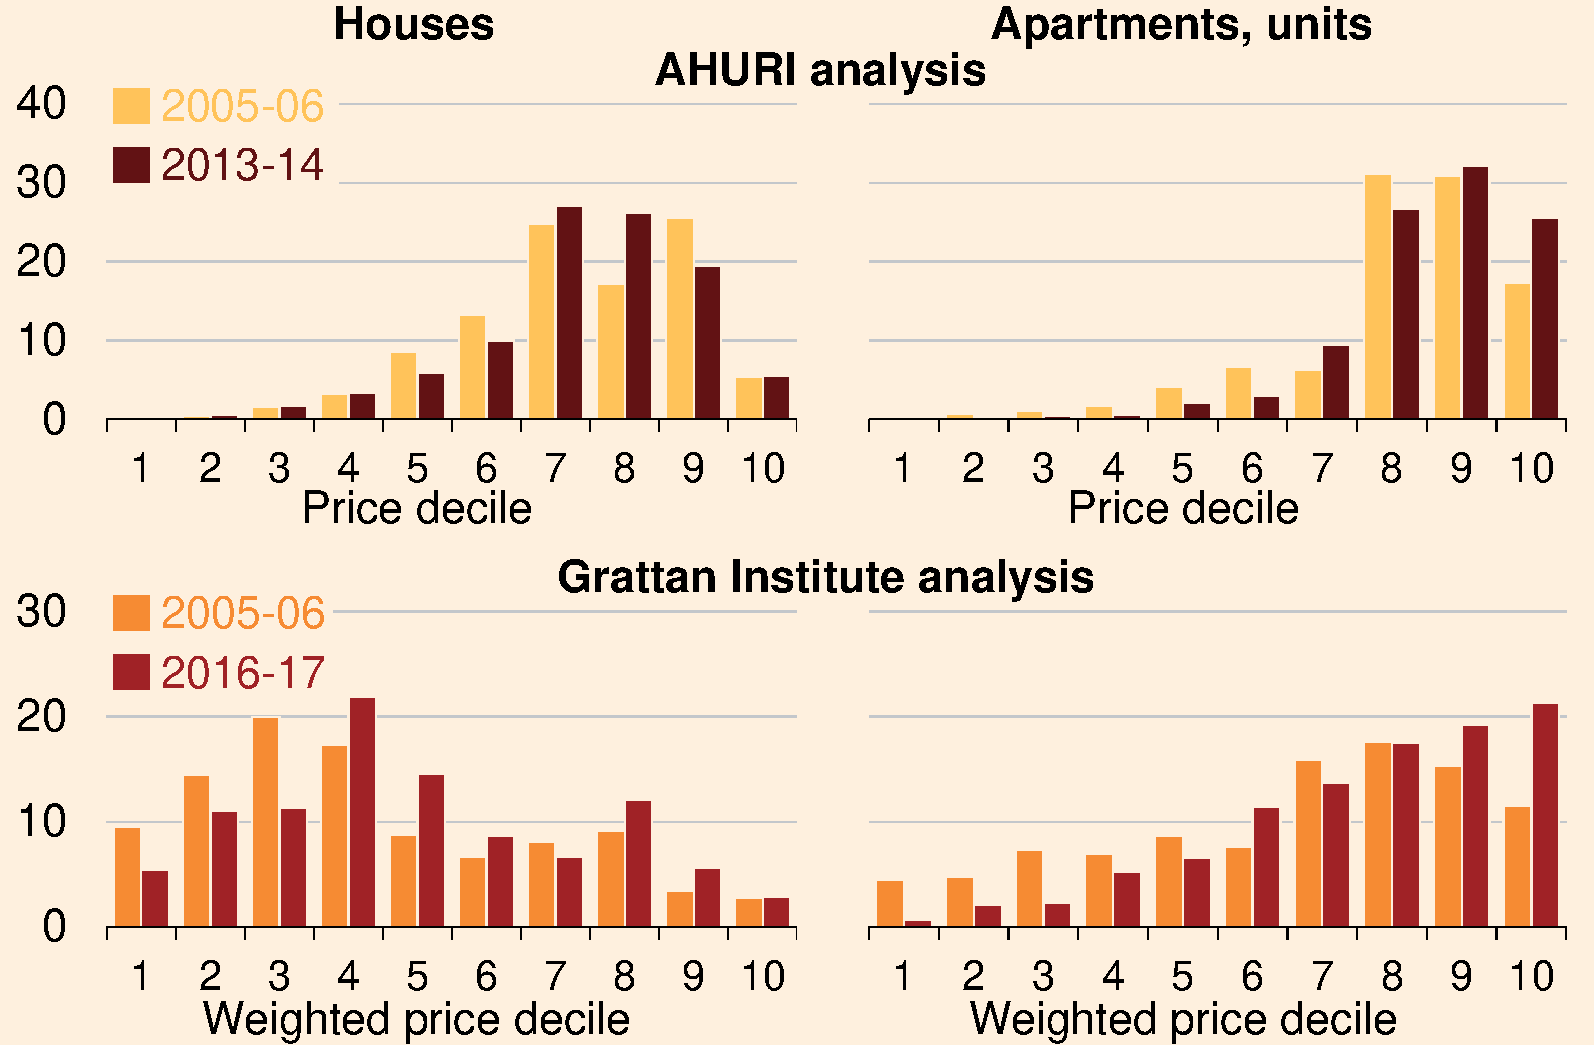
\includegraphics[page=1]{atlas/Approvals_by_weighted_price_decile_long.pdf}
		\noteswithsource{Weighted price deciles are calculated by ranking LGAs according to their median price values, and sorting into deciles weighted by the total dwelling stock in each LGA so that each decile has a similar number of dwellings (LGAs without price data were excluded). All building approvals for an LGA are assigned to the decile that it sits in. LGAs are as they were in 2006 and 2016, with the best available price data assigned to that LGA (some very small LGAs were excluded). `Apartments, units' includes units, apartments, flats, semi-detached, row or terrace houses and townhouses in Grattan analysis. This is consistent with the definition of the CoreLogic price data used to rank LGAs by median house and unit price. In contrast, \textcite{OngEtAl-AHURI-2017-Housing-supply-responsiveness} appear to include semi-detached and townhouses in the `Houses' category.}{\textcites{OngEtAl-AHURI-2017-Housing-supply-responsiveness}{ABS-2017-Building-approvals-Sep-2015}{ABS20016Censuspopulationhousing}{ABS2006}; Grattan analysis based on CoreLogic data.}
		\end{figure}
		
\end{bigbox*}

And even if new housing were biased towards more expensive dwellings, it would still `filter down' to improve affordability for lower-income households.
More housing supply -- even if priced at the top end -- should ultimately free-up less expensive housing stock.
The people who move into newly constructed more expensive housing are either existing residents who move out of less expensive housing, or new residents who would otherwise have added to the demand and pushed up the price of existing housing.
Irrespective of its cost, each additional dwelling adds to total supply, which ultimately affects affordability for all home buyers.%
	\footnote{While gentrification can push up prices in a particular area, the construction of additional housing in total should lead to prices being lower than otherwise overall.}

There is good international evidence to suggest that this `filtering' does occur in practice.
Initially expensive homes gradually become cheaper as they age, and are sold or rented to people with more modest incomes, and this is a strong source of more affordable housing, especially in the private rental market.%
	\footnote{For example, \textcite{Rosenthal2014PrivateMarkets} finds that the US housing stock `filters' by roughly 1.9 per cent a year -- meaning that a 50-year-old home is typically occupied by someone whose income is about 60 per cent lower than that home's first occupant.
	Most of the filtering of once high-end housing to lower-income groups occurs within the first 20 years of a dwelling's life.
	See also \textcite{Taylor2016Perspectives}; \textcite{Somerville-Mayer-2003-govt-reg-affordable-housing}.}
US estimates suggest that 45 per cent of homes that were affordable to very low-income earners in the United States in 2013 had filtered down from owner-occupier or higher rent categories in 1985.%
    \footnote{\textcite{Weicheretal-The-Long-Term-Dynamics-of-Affordable-Rental-Housing}. The authors define affordable housing as rentals that cost no more than 30 per cent of income for households with 50 per cent or less of the median income for the area.}

Of course, if new construction is disproportionately more expensive, then the overall housing stock will become more expensive -- but this ultimately merely reflects choices across the market to spend more on housing in preference to other goods and services.

New expensive housing might not improve the balance between supply and demand if it merely induced additional demand, presumably from overseas purchasers.
But, as discussed above (See \Cref{subsec:tax-settings-encourage-people-to-invest-in-housing}), there is little evidence that overseas purchasers are increasing demand by much more than they increase supply, and even less evidence that they are the \emph{only} purchasers of more expensive housing.

Similarly, filtering may not work effectively if house prices more broadly are rising quickly. For example, \textcite{AHURI-2011-affordable-rental} found that housing was only affordable for 37 per cent of private renters with household incomes in the lowest 40 per cent of the national income distribution in 2006.%
    \footnote{Of course, this hinges on the arbitrary definition of `affordable': the typical household in the bottom 20 per cent of incomes spends 28 per cent of its income on housing (\Vref{fig:spending-on-housing-by-income}). \textcite{AHURI-2011-affordable-rental}
    defined private rental as `affordable' if it cost no more than 30 per cent of the income of households in the bottom two income quintiles.}
New -- or old -- housing is unlikely to become more accessible to low-income earners in a world where overall house prices are rising rapidly, especially if overall housing supply falls behind population growth because of restrictive land use planning rules. This underscores the need for broader reforms to boost housing supply to improve affordability.%
    \footnote{For example, \textcite{Somerville-Mayer-2003-govt-reg-affordable-housing} find that restrictions on the supply of new units lower the supply of affordable units. More demand for higher quality units increases the incentives for landlords to upgrade existing units into a higher quality, higher return housing sub-market.}

While more market housing can make housing more affordable for all Australians, including many low-income earners, some level of subsidies will always be required so that those worst off can afford housing (\Vref{sec:helping-the-bottom}). But making housing cheaper overall will reduce the amount of public subsidy needed to bridge the gap between the market price of housing and what low-income earners can afford to pay.%
    \footcite[][1]{Daley-etal-2017-Submission-Natl-housing-finance}

% TODO: put between page 58 & 59
\clearpage
% \pagestyle{empty}
% 	\pagecolor{OrangeBackground}
	\begin{boxshell}
	\begin{leftfullpage}
	  \begin{mdframed}[style=GrattanFrameBoxA]
	    \captionsetup{labelfont       = {bf, Orange},
		                font            = {bf, Orange},
		                format          = plain,
		                justification   = raggedright,
		                singlelinecheck = false,
		                skip            = 0ex,
		                position        = above}
		  \dummyCaption{The Victorian planning system restricts the supply of new housing and contributes to higher prices\label{box:Victoria-planning-applications}}
		  \captionsetup{format    = plain,
		                font      = {small, bf, theGrey},
		                labelfont = {small, bf, theGrey},
		                position  = above,
		                skip      = 0pt}
		  % Reduced column sep
		  \addtolength{\columnsep}{-23.8pt}%
		  %\pagecolor{OrangeBackground}
		  \begin{multicols}{2}
			  \setlength{\parskip}{4pt plus 1pt minus 1pt}
			  \RaggedRight
				Our analysis of planning approvals in Victoria between 2007 and 2017 shows that the planning approval process is lengthy and costly to developers, and increases prices for home-buyers.%
				  \footnote{\textcite[][402]{Gurran_Phibbs_2013_housing_supply} also find that, `Victoria’s planning system would seem to be far slower and less certain than those of the other jurisdictions'.}
				Dwelling development applications face substantial delays in inner and middle-ring Melbourne council areas, where housing is in greatest demand.
				The typical dwelling application takes over 214 days%
				  \footnote{The median number of days to finalisation for applications that are granted
				  either by council or through VCAT, excluding applications that are not finalised or not granted.
				  Some of the additional time taken may be due to increased complexity of the application, but
				  single dwelling applications, which are typically less complex, also take longer to get approved in most inner-city councils.}
				to get approved in the City of Melbourne, and longer in Port Phillip and Yarra councils (see \Cref{fig:Melb_planning_map}).
				The approvals process is typically much faster in growth area councils.


				Councils where residents are more politically active may be more reluctant to approve development. They have scope to do so in part because the Victorian planning system aims to protect `neighbourhood character,' which is an inherently vague criterion open to differing interpretations.%
				    \footcites{VICDepLWP2017Neighbour}[][64, 72, 91]{Rowley_2017_Vic_planning_system}

				Inner city councils appear to delay development by a similar amount. In addition to the restrictions within their own planning schemes, some councils seem to use different strategies in the application process to delay development. These are reflected by developers tending to use different grounds for applying to VCAT for review in different council areas.
				Port Phillip is more likely to fail to decide within the prescribed time, whereas Glen Eira is more likely to initially reject an application (\Cref{fig:Melb_planning_delays_chart}).

				\begin{figure}[H]
				\caption{Permits take longer for dwelling development applications in inner and middle ring council areas}\label{fig:Melb_planning_map}
				\units{Median days to permit approval for single and multiple dwelling applications by suburb with LGA boundaries, 2007-2017}
				\includegraphics[page=2]{atlas/Melb_planning_delays_map_short.pdf}
				\noteswithsource{Excludes dwellings that do not require a development application. Does not include the time taken if there were multiple applications for the same dwelling}{Grattan analysis of Victorian Planning Permit Activity Reporting System 2017}
				\end{figure}
			\end{multicols}
		\end{mdframed}
	\end{leftfullpage}
	\end{boxshell}
	\begin{boxshell}
	\begin{fullpage}
% 	\pagecolor{OrangeBackground}
	  \begin{mdframed}[style=GrattanFrameBoxB]
	  \captionsetup{labelfont       = {bf, Orange},
	                font            = {bf, Orange},
	                format          = plain,
	                justification   = raggedright,
	                singlelinecheck = false,
	                skip            = 0ex,
	                position        = above}
% 	  \caption*{Box \ref{box:Victoria-planning-applications} (continued): \nameref{box:Victoria-planning-applications}}%
	  \captionsetup{format    = plain,
	                font      = {small, bf, theGrey},
	                labelfont = {small, bf, theGrey},
	                position  = above,
	                skip      = 0pt}
    \addtolength{\columnsep}{-23.8pt}%
	  \begin{multicols}{2}
	  \setlength{\parskip}{4pt plus 1pt minus 1pt}
	  \RaggedRight

		Victoria's planning system is more open to third party reviews than other jurisdictions, and so a higher proportion of planning decisions are reviewed than in NSW.%
		    \textsuperscript{d}

		Development applications in inner city areas are more likely than outer suburban applications to be reviewed by the Victorian Civil and Administrative Tribunal (VCAT). Applications that are reviewed typically take much longer to be finalised.%
			\textsuperscript{e}

		Almost a third of all local council assessed dwelling applications go to VCAT in Melbourne, Port Phillip and Yarra councils. By contrast, less than five per cent go to VCAT in growth area councils (see \Cref{fig:Melb_planning_delays_chart}).%
			\textsuperscript{f}
        These applications are not frivolous: in both Port Phillip and Yarra, the majority ultimately receive development approval.%
        	\textsuperscript{g}

        The delay involved in applying to VCAT increases costs and uncertainty for developers, which are often passed on to purchasers. A slower supply of new dwellings also increases prices (\eg~see \textcite{Mayer_Somerville_2000_land_use_regulation} and \Vref{box:International-supply-literature}).


		\rule{0.2\columnwidth}{0.4pt}\linebreak
		\begin{tabularx}{\columnwidth}{@{}>{\centering\footnotesize}p{1.5em}@{}>{\footnotesize\arraybackslash}X}
		d.~\null &
		    {39 per cent of all Victorian permit applications received were advertised to third parties and 4 per cent were reviewed by VCAT in 2014-15.
		    In NSW, third party objectors must have a `relevant interest' in the development.
		    In 2014-15, less than 1 per cent, of the 106,077 permit applications received were reviewed or appealed (\textcite[][28]{PC-2017-shifting-dial-potential-of-land}).} \\
		e.~\null &
		    {Within inner and middle Melbourne, applications that are approved by council typically take 116 days for single-dwelling applications and 156 for multiple-dwelling applications. But applications that go to VCAT typically take over a year before they are finalised.} \\
		f.~\null &
            {In Port Phillip 83 per cent of applications were granted when taken to VCAT by the developer for failing to decide within the prescribed time.
			In Glen Eira 62 per cent of applications were granted when taken to VCAT by the developer to contest the council’s refusal to grant a permit.} \\
		g.~\null &
            {Of applications to VCAT by developers between 2015 and mid-2017 and decided by mid-2017, the developer succeeded in 86 per cent of cases when they contested some or all of the council's conditions on development, and in 66 per cent of cases when they contested council's outright rejection.
            But developer success at VCAT reflects survivorship bias: most development applications rejected by council are not taken to VCAT.} \\

		\end{tabularx}


		\begin{figure}[H]
		\caption{Dwelling development applications are more likely to go to VCAT in inner and middle ring council areas}\label{fig:Melb_planning_delays_chart}
		\units{Proportion of finalised dwelling applications taken to VCAT 2015-2017}
		\includegraphics[page=2]{atlas/Melb_planning_delays_chart_long.pdf}
		\noteswithsource{Applications to VCAT by objectors are slightly under-represented because when both developer and objectors applied to VCAT, the proposal was classified as a developer application. Only includes applications where the local council was the responsible authority. Excludes applications that had not been finalised by mid-2017 (so the proportion of dwelling applications taken to VCAT between 2007 and 2017 is typically about 5 percentage points higher than shown).}{Grattan analysis of Victorian Planning Permit Activity Reporting System 2017}
		\end{figure}
		\end{multicols}
	  \end{mdframed}
  \end{fullpage}
  \end{boxshell}
\clearpage\nopagecolor
% \pagestyle{scrheadings}
